% "{'classe':('PSI'),'chapitre':'dyn_pfd','type':('cours'),'titre':'Dynamique du solide indéformable', 'source':' ','comp':('DYN-01','DYN-02','DYN-03','DYN-04'),'corrige':True}"
\setchapterimage{Fond_CIN.png}
\setchapterpreamble[u]{\margintoc}
%\setcounter{chapter}{1}

\chapter{Cours de dynamique du solide indéformable}

\marginnote{\xpComp{DYN}{01}\xpComp{DYN}{02}\xpComp{DYN}{03}\xpComp{DYN}{04}}
%


%\documentclass[10pt,fleqn]{article} % Default font size and left-justified equations
%\usepackage[%
%    pdftitle={Equilibrage des solides en rotation},
%    pdfauthor={Xavier Pessoles}]{hyperref}
%
%%%%%%%%%%%%%%%%%%%%%%%%%%%%%%%%%%%%%%%%%%
% Original author:
% Mathias Legrand (legrand.mathias@gmail.com) with modifications by:
% Vel (vel@latextemplates.com)
% X Pessoles xpessoles.ptsi@free.fr
% License:
% CC BY-NC-SA 3.0 (http://creativecommons.org/licenses/by-nc-sa/3.0/)
%%%%%%%%%%%%%%%%%%%%%%%%%%%%%%%%%%%%%%%%%

%----------------------------------------------------------------------------------------
%	VARIOUS REQUIRED PACKAGES AND CONFIGURATIONS
%----------------------------------------------------------------------------------------

\usepackage[top=2.5cm,bottom=2cm,left=2cm,right=2cm,headsep=40pt,a4paper]{geometry} % Page margins

\usepackage{graphicx} % Required for including pictures
\graphicspath{{images/}} % Specifies the directory where pictures are stored

\usepackage{lipsum} % Inserts dummy text

\usepackage{tikz} % Required for drawing custom shapes

\usepackage[french]{babel} % English language/hyphenation
\frenchbsetup{StandardLists=true} % Pour éviter la collision babel enumitem pour les listes

\usepackage{enumitem} % Customize lists
\setlist{nolistsep} % Reduce spacing between bullet points and numbered lists

\usepackage{booktabs} % Required for nicer horizontal rules in tables

\usepackage{xcolor} % Required for specifying colors by name
%\definecolor{ocre}{RGB}{243,102,25} % Define the orange color used for highlighting throughout the book
 \definecolor{ocre}{RGB}{49,133,156} % Couleur ''bleue''
\definecolor{violetf}{RGB}{112,48,160} % Couleur ''violet''
\usepackage{enumitem}
\usepackage{pifont} % Pour les dinglist
\usepackage{multicol}
\usepackage{array} % Centrage vertical dans les tableaux



% DIVERS STANDALONE + TIKZ
%%%%%%%%%%%%%%%%%%%
\usepackage{numprint}
\usetikzlibrary{calc}
\usepackage{siunitx}
%definition style pour mettre un fond blanc dans un node sans avoir des marges énormes
\tikzset{fondblanc/.style={ inner sep=2pt,fill=white,outer sep = 5pt}} 
\tikzset{fondblanc2/.style={ inner sep=2pt,fill=white}} 
\tikzset{fondblanc3/.style={ inner sep=1pt,fill=white,outer sep = 2pt}} 
%\usetikzlibrary{calc,circuits.ee.IEC}
%\usetikzlibrary{shapes}
%\usepackage[european resistor, european voltage, european current]{circuitikz}
%\usetikzlibrary{babel}
\usepackage{standalone}
\standaloneconfig{mode=buildnew}





%----------------------------------------------------------------------------------------
%	FONTS
%----------------------------------------------------------------------------------------

\usepackage{avant} % Use the Avantgarde font for headings
%\usepackage{times} % Use the Times font for headings
%\usepackage{mathptmx} % Use the Adobe Times Roman as the default text font together with math symbols from the Sym­bol, Chancery and Com­puter Modern fonts
\usepackage[adobe-utopia]{mathdesign}
\usepackage{microtype} % Slightly tweak font spacing for aesthetics
\usepackage[utf8]{inputenc} % Required for including letters with accents
\usepackage[T1]{fontenc} % Use 8-bit encoding that has 256 glyphs

%----------------------------------------------------------------------------------------
%	BIBLIOGRAPHY AND INDEX
%----------------------------------------------------------------------------------------

\usepackage[style=alphabetic,citestyle=numeric,sorting=nyt,sortcites=true,autopunct=true,babel=hyphen,hyperref=true,abbreviate=false,backref=true,backend=biber]{biblatex}
\addbibresource{bibliography.bib} % BibTeX bibliography file
\defbibheading{bibempty}{}

\usepackage{calc} % For simpler calculation - used for spacing the index letter headings correctly
\usepackage{makeidx} % Required to make an index
\makeindex % Tells LaTeX to create the files required for indexing

%----------------------------------------------------------------------------------------
%	MAIN TABLE OF CONTENTS
%----------------------------------------------------------------------------------------

\usepackage{titletoc} % Required for manipulating the table of contents

\setcounter{tocdepth}{2}     % Dans la table des matieres
\setcounter{secnumdepth}{2}

\contentsmargin{0cm} % Removes the default margin

% Part text styling
\titlecontents{part}[0cm]
{\addvspace{20pt}\centering\large\bfseries}
{}
{}
{}

% Chapter text styling
\titlecontents{chapter}[1.25cm] % Indentation
{\addvspace{12pt}\large\sffamily\bfseries} % Spacing and font options for chapters
{\color{ocre!60}\contentslabel[\Large\thecontentslabel]{1.25cm}\color{ocre}} % Chapter number
{\color{ocre}}  
{\color{ocre!60}\normalsize\;\titlerule*[.5pc]{.}\;\thecontentspage} % Page number

% Section text styling
\titlecontents{section}[1.25cm] % Indentation
{\addvspace{3pt}\sffamily\bfseries} % Spacing and font options for sections
{\color{ocre!60}\contentslabel[\thecontentslabel]{1.25cm} \color{ocre}} % Section number
{\color{ocre}}
{\hfill\color{ocre!60}\thecontentspage} % Page number
[]

% Subsection text styling
\titlecontents{subsection}[1.25cm] % Indentation
{\addvspace{1pt}\sffamily\small} % Spacing and font options for subsections
{\contentslabel[\thecontentslabel]{1.25cm}} % Subsection number
{}
{\ \titlerule*[.5pc]{.}\;\thecontentspage} % Page number
[]


% Subsection text styling
\titlecontents{subsubsection}[1.25cm] % Indentation
{\addvspace{1pt}\sffamily\small} % Spacing and font options for subsections
{\contentslabel[\thecontentslabel]{1.25cm}} % Subsection number
{}
{\ \titlerule*[.5pc]{.}\;\thecontentspage} % Page number
[]

% List of figures
\titlecontents{figure}[0em]
{\addvspace{-5pt}\sffamily}
{\thecontentslabel\hspace*{1em}}
{}
{\ \titlerule*[.5pc]{.}\;\thecontentspage}
[]

% List of tables
\titlecontents{table}[0em]
{\addvspace{-5pt}\sffamily}
{\thecontentslabel\hspace*{1em}}
{}
{\ \titlerule*[.5pc]{.}\;\thecontentspage}
[]

%----------------------------------------------------------------------------------------
%	MINI TABLE OF CONTENTS IN PART HEADS
%----------------------------------------------------------------------------------------

% Chapter text styling
\titlecontents{lchapter}[0em] % Indenting
{\addvspace{15pt}\large\sffamily\bfseries} % Spacing and font options for chapters
{\color{ocre}\contentslabel[\Large\thecontentslabel]{1.25cm}\color{ocre}} % Chapter number
{}  
{\color{ocre}\normalsize\sffamily\bfseries\;\titlerule*[.5pc]{.}\;\thecontentspage} % Page number

% Section text styling
\titlecontents{lsection}[0em] % Indenting
{\sffamily\small} % Spacing and font options for sections
{\contentslabel[\thecontentslabel]{1.25cm}} % Section number
{}
{}

% Subsection text styling
\titlecontents{lsubsection}[.5em] % Indentation
{\normalfont\footnotesize\sffamily} % Font settings
{}
{}
{}

%----------------------------------------------------------------------------------------
%	PAGE HEADERS
%----------------------------------------------------------------------------------------

\usepackage{fancyhdr} % Required for header and footer configuration



\pagestyle{fancy}
 \renewcommand{\headrulewidth}{0pt}
 \fancyhead{}
 \fancyhead[L]{%
 \noindent\begin{minipage}[c]{2.6cm}%
 
\includegraphics[width=2cm]{png/logo_lycee.png}%
 \end{minipage}}

\fancyhead[C]{\rule{8cm}{.5pt}}

 \fancyhead[R]{%
 \noindent\begin{minipage}[c]{3cm}
 \begin{flushright}
 \footnotesize{\textit{\textsf{\xxtete}}}%
 \end{flushright}
 \end{minipage}
}


\fancyfoot[C]{\rule{12cm}{.5pt}}
\renewcommand{\footrulewidth}{0.2pt}
\fancyfoot[C]{\footnotesize{\bfseries \thepage}}
\fancyfoot[L]{ 
\begin{minipage}[c]{.4\linewidth}
\noindent\footnotesize{{\xxauteur}}
\end{minipage}}


\fancyfoot[R]{\footnotesize{\xxpied}
\ifthenelse{\isodd{\value{page}}}{
\begin{tikzpicture}[overlay]
\node[shape=rectangle, 
      rounded corners = .25 cm,
	  draw= ocre,
	  line width=2pt, 
	  fill = ocre!10,
	  minimum width  = 2.5cm,
	  minimum height = 3cm,] at (\xxposongletx,\xxposonglety) {};
\node at (\xxposonglettext,\xxposonglety) {\rotatebox{90}{\textbf{\large\color{ocre}{\xxonglet}}}};
%{};
\end{tikzpicture}}{}
}
%
%
%
% Removes the header from odd empty pages at the end of chapters
\makeatletter
\renewcommand{\cleardoublepage}{
\clearpage\ifodd\c@page\else
\hbox{}
\vspace*{\fill}
\thispagestyle{empty}
\newpage
\fi}

\fancypagestyle{plain}{%
\fancyhf{} % vide l’en-tête et le pied~de~page.
%\fancyfoot[C]{\bfseries \thepage} % numéro de la page en cours en gras
% et centré en pied~de~page.
\fancyfoot[R]{\footnotesize{\xxpied}}
\fancyfoot[C]{\rule{12cm}{.5pt}}
\renewcommand{\footrulewidth}{0.2pt}
\fancyfoot[C]{\footnotesize{\bfseries \thepage}}
\fancyfoot[L]{ 
\begin{minipage}[c]{.4\linewidth}
\noindent\footnotesize{{\xxauteur}}
\end{minipage}}}



%----------------------------------------------------------------------------------------
%	THEOREM STYLES
%----------------------------------------------------------------------------------------

% Conflit avec la police adobe
%\usepackage{amsmath,amsfonts,amssymb,amsthm} % For math equations, theorems, symbols, etc
\usepackage{amsmath,amsthm}

\newcommand{\intoo}[2]{\mathopen{]}#1\,;#2\mathclose{[}}
\newcommand{\ud}{\mathop{\mathrm{{}d}}\mathopen{}}
\newcommand{\intff}[2]{\mathopen{[}#1\,;#2\mathclose{]}}
%\newtheorem{notation}{Notation}[chapter]
\newtheorem{notation}{Notation}[section]

% Boxed/framed environments
\newtheoremstyle{ocrenumbox}% % Theorem style name
{0pt}% Space above
{0pt}% Space below
{\normalfont}% % Body font
{}% Indent amount
{\small\bf\sffamily\color{ocre}}% % Theorem head font
{\;}% Punctuation after theorem head
{0.25em}% Space after theorem head
{\small\sffamily\color{ocre}\thmname{#1}\nobreakspace\thmnumber%{\@ifnotempty{#1}{}\@upn{#2}}% Theorem text (e.g. Theorem 2.1)
\thmnote{\nobreakspace\the\thm@notefont\sffamily\bfseries\color{black}---\nobreakspace#3.}} % Optional theorem note
\renewcommand{\qedsymbol}{$\blacksquare$}% Optional qed square


% Boite pour les corriges
\newtheoremstyle{correctionbox}% % Theorem style name
{0pt}% Space above
{0pt}% Space below
{\normalfont}% % Body font
{}% Indent amount
{\small\bf\sffamily\color{violet}}% % Theorem head font
{\;}% Punctuation after theorem head
{0.25em}% Space after theorem head
{\small\sffamily\color{ocre}\thmname{#1}\nobreakspace\thmnumber%{\@ifnotempty{#1}{}\@upn{#2}}% Theorem text (e.g. Theorem 2.1)
\thmnote{\nobreakspace\the\thm@notefont\sffamily\bfseries\color{black}---\nobreakspace#3.}} % Optional theorem note
\renewcommand{\qedsymbol}{$\blacksquare$}% Optional qed square



\newtheoremstyle{blacknumex}% Theorem style name
{5pt}% Space above
{5pt}% Space below
{\normalfont}% Body font
{} % Indent amount
{\small\bf\sffamily}% Theorem head font
{\;}% Punctuation after theorem head
{0.25em}% Space after theorem head
{\small\sffamily{\tiny\ensuremath{\blacksquare}}\nobreakspace\thmname{#1}\nobreakspace\thmnumber%{\@ifnotempty{#1}{}\@upn{#2}}% Theorem text (e.g. Theorem 2.1)
\thmnote{\nobreakspace\the\thm@notefont\sffamily\bfseries---\nobreakspace#3.}}% Optional theorem note

\newtheoremstyle{blacknumbox} % Theorem style name
{0pt}% Space above
{0pt}% Space below
{\normalfont}% Body font
{}% Indent amount
{\small\bf\sffamily}% Theorem head font
{\;}% Punctuation after theorem head
{0.25em}% Space after theorem head
{\small\sffamily\thmname{#1}\nobreakspace 
\thmnote{\nobreakspace\the\thm@notefont\sffamily\bfseries---\nobreakspace#3.}}% Optional theorem note

% Non-boxed/non-framed environments
\newtheoremstyle{ocrenum}% % Theorem style name
{5pt}% Space above
{5pt}% Space below
{\normalfont}% % Body font
{}% Indent amount
{\small\bf\sffamily\color{ocre}}% % Theorem head font
{\;}% Punctuation after theorem head
{0.25em}% Space after theorem head
{\small\sffamily\color{ocre}\thmname{#1}\nobreakspace%\thmnumber{\@ifnotempty{#1}{}\@upn{#2}}% Theorem text (e.g. Theorem 2.1)
\thmnote{\nobreakspace\the\thm@notefont\sffamily\bfseries\color{black}---\nobreakspace#3.}} % Optional theorem note
\renewcommand{\qedsymbol}{$\blacksquare$}% Optional qed square
\makeatother

% Environnement pour les titres de parties
\newtheoremstyle{partiebox} 
{0pt}% Space above
{0pt}% Space below
{\normalfont}% Body font
{}% Indent amount
{\small\bf\sffamily}% Theorem head font
{\;}% Punctuation after theorem head
{0.25em}% Space after theorem head




% Defines the theorem text style for each type of theorem to one of the three styles above
\newcounter{dummy} 
\numberwithin{dummy}{section}
\theoremstyle{ocrenumbox}
%\newtheorem{theoremeT}[dummy]{Théorème}
\newtheorem{theoremeT}[dummy]{Théorème}
\newtheorem{resultatT}[dummy]{Résultat}
\newtheorem{savoirT}[dummy]{Savoir}
\newtheorem{methodeT}[dummy]{Méthode}
\newtheorem{objectifT}[dummy]{Objectif}
%\newtheorem{problem}{Problem}[chapter]
\newtheorem{problem}{Problem}[section]
%\newtheorem{exerciseT}{Exercise}[chapter]
\newtheorem{exerciseT}{Exercice}[section]

\theoremstyle{blacknumex}
%\newtheorem{exampleT}{Example}[chapter]
\newtheorem{exempleT}{Exemple}[section]
\newtheorem{termT}{Terminal\\}[section]
\newtheorem{pyT}{Python\\}[section]
\newtheorem{sciT}{Scilab\\}[section]
\newtheorem{pseudoT}{Pseudo Code\\}[section]
\newtheorem{sqlT}{SQL\\}[section]

\theoremstyle{blacknumbox}
%\newtheorem{vocabulary}{Vocabulary}[chapter]
\newtheorem{vocabulary}{Vocabulaire}[section]
%\newtheorem{definitionT}{Definition}[section]
\newtheorem{definitionT}{Définition}[section]
\newtheorem{propT}{Propriété}[section]
\newtheorem{rappelT}{Rappel}[section]
\newtheorem{demoT}{Démonstration}[section]
\newtheorem{corollaryT}[dummy]{Corollaire}
\newtheorem{hypoT}{Hypothèse(s)}

\theoremstyle{ocrenum}
\newtheorem{proposition}[dummy]{Proposition}

\theoremstyle{partiebox}
\newtheorem{titrepartieT}[]{}
\newtheorem{titrechapitreT}[]{}

\theoremstyle{correctionbox}
\newtheorem{correctionT}[dummy]{\color{violet}{Correction}}

%----------------------------------------------------------------------------------------
%	DEFINITION OF COLORED BOXES
%----------------------------------------------------------------------------------------

\RequirePackage[framemethod=tikz]{mdframed} % Required for creating the theorem, definition, exercise and corollary boxes

% Theorem box
\newmdenv[skipabove=7pt,
skipbelow=7pt,
backgroundcolor=ocre!10,
linecolor=ocre,
innerleftmargin=5pt,
innerrightmargin=5pt,
innertopmargin=5pt,
leftmargin=0cm,
rightmargin=0cm,
innerbottommargin=5pt]{tBox}


% Correction
\newmdenv[skipabove=7pt,
skipbelow=7pt,
backgroundcolor=violet!10,
linecolor=violet,
innerleftmargin=5pt,
innerrightmargin=5pt,
innertopmargin=5pt,
leftmargin=0cm,
rightmargin=0cm,
innerbottommargin=5pt]{coBox}


% Exercise box	  
\newmdenv[skipabove=7pt,
skipbelow=7pt,
rightline=false,
leftline=true,
topline=false,
bottomline=false,
backgroundcolor=ocre!10,
linecolor=ocre,
innerleftmargin=5pt,
innerrightmargin=5pt,
innertopmargin=5pt,
innerbottommargin=5pt,
leftmargin=0cm,
rightmargin=0cm,
linewidth=4pt]{eBox}	

% Definition box
\newmdenv[skipabove=7pt,
skipbelow=7pt,
rightline=false,
leftline=true,
topline=false,
bottomline=false,
backgroundcolor=ocre!10,
linecolor=ocre,
innerleftmargin=5pt,
innerrightmargin=5pt,
innertopmargin=0pt,
leftmargin=0cm,
rightmargin=0cm,
linewidth=4pt,
innerbottommargin=0pt]{dBox}	

% Demonstration box
\newmdenv[skipabove=7pt,
skipbelow=7pt,
rightline=false,
leftline=true,
topline=false,
bottomline=false,
%backgroundcolor=ocre!10,
linecolor=ocre,
innerleftmargin=5pt,
innerrightmargin=5pt,
innertopmargin=0pt,
leftmargin=0cm,
rightmargin=0cm,
linewidth=4pt,
innerbottommargin=0pt]{demoBox}	

% Corollary box
\newmdenv[skipabove=7pt,
skipbelow=7pt,
rightline=false,
leftline=true,
topline=false,
bottomline=false,
linecolor=gray,
backgroundcolor=black!5,
innerleftmargin=5pt,
innerrightmargin=5pt,
innertopmargin=5pt,
leftmargin=0cm,
rightmargin=0cm,
linewidth=4pt,
innerbottommargin=5pt]{cBox}


% Hypothèses
\newmdenv[skipabove=7pt,
skipbelow=7pt,
rightline=false,
leftline=true,
topline=false,
bottomline=false,
linecolor=gray,
backgroundcolor=black!5,
innerleftmargin=5pt,
innerrightmargin=5pt,
innertopmargin=1pt,
leftmargin=0cm,
rightmargin=0cm,
linewidth=4pt,
innerbottommargin=1pt]{hyBox}


% Boite pour le titre de la partie (pBox)
\newmdenv[skipabove=7pt,
skipbelow=7pt,
rightline=true,
leftline=false,
topline=false,
bottomline=false,
linecolor=ocre,
backgroundcolor=none,
innerleftmargin=5pt,
innerrightmargin=5pt,
innertopmargin=5pt,
leftmargin=0cm,
rightmargin=0cm,
linewidth=4pt,
innerbottommargin=5pt]{pBox}

% Boite pour le titre du chapitre (chBox)
\newmdenv[skipabove=7pt,
skipbelow=7pt,
rightline=false,
leftline=true,
topline=false,
bottomline=false,
linecolor=ocre,
%backgroundcolor=black!5,
innerleftmargin=5pt,
innerrightmargin=5pt,
innertopmargin=5pt,
leftmargin=0cm,
rightmargin=0cm,
linewidth=4pt,
innerbottommargin=5pt]{chBox}


% Boite pour les exemples
\newmdenv[skipabove=7pt,
skipbelow=7pt,
rightline=false,
leftline=true,
topline=false,
bottomline=false,
linecolor=gray,
backgroundcolor=white,
innerleftmargin=5pt,
innerrightmargin=5pt,
innertopmargin=5pt,
leftmargin=0cm,
rightmargin=0cm,
linewidth=4pt,
innerbottommargin=5pt]{exBox}

% Boite pour le terminal
\newmdenv[skipabove=7pt,
skipbelow=7pt,
rightline=false,
leftline=true,
topline=false,
bottomline=false,
linecolor=gray,
backgroundcolor=white,
innerleftmargin=5pt,
innerrightmargin=5pt,
innertopmargin=5pt,
leftmargin=0cm,
rightmargin=0cm,
linewidth=4pt,
innerbottommargin=5pt]{termBox}


% Boite pour Python
\newmdenv[skipabove=7pt,
skipbelow=7pt,
rightline=false,
leftline=true,
topline=false,
bottomline=false,
linecolor=gray,
backgroundcolor=white,
innerleftmargin=5pt,
innerrightmargin=5pt,
innertopmargin=0pt,
leftmargin=0cm,
rightmargin=0cm,
linewidth=4pt,
innerbottommargin=5pt]{pyBox}

% Boite pour scilab
\newmdenv[skipabove=7pt,
skipbelow=7pt,
rightline=false,
leftline=true,
topline=false,
bottomline=false,
linecolor=gray,
backgroundcolor=white,
innerleftmargin=5pt,
innerrightmargin=5pt,
innertopmargin=5pt,
leftmargin=0cm,
rightmargin=0cm,
linewidth=4pt,
innerbottommargin=5pt]{sciBox}


% Boite pour pseudo
\newmdenv[skipabove=7pt,
skipbelow=7pt,
rightline=false,
leftline=true,
topline=false,
bottomline=false,
linecolor=gray,
backgroundcolor=white,
innerleftmargin=5pt,
innerrightmargin=5pt,
innertopmargin=5pt,
leftmargin=0cm,
rightmargin=0cm,
linewidth=4pt,
innerbottommargin=5pt]{pseudoBox}

% Boite pour pseudo
\newmdenv[skipabove=7pt,
skipbelow=7pt,
rightline=false,
leftline=true,
topline=false,
bottomline=false,
linecolor=gray,
backgroundcolor=white,
innerleftmargin=5pt,
innerrightmargin=5pt,
innertopmargin=5pt,
leftmargin=0cm,
rightmargin=0cm,
linewidth=4pt,
innerbottommargin=5pt]{sqlBox}


% Creates an environment for each type of theorem and assigns it a theorem text style from the "Theorem Styles" section above and a colored box from above
\newenvironment{theorem}{\begin{tBox}\begin{theoremeT}}{\end{theoremeT}\end{tBox}}
\newenvironment{resultat}{\begin{tBox}\begin{resultatT}}{\end{resultatT}\end{tBox}}
\newenvironment{methode}{\begin{tBox}\begin{methodeT}}{\end{methodeT}\end{tBox}}
\newenvironment{savoir}{\begin{tBox}\begin{savoirT}}{\end{savoirT}\end{tBox}}
\newenvironment{obj}{\begin{tBox}\begin{objectifT}}{\end{objectifT}\end{tBox}}
\newenvironment{corrige}{\begin{coBox}\begin{correctionT}}{\end{correctionT}\end{coBox}}
\newenvironment{exercise}{\begin{eBox}\begin{exerciseT}}{\hfill{\color{ocre}\tiny\ensuremath{\blacksquare}}\end{exerciseT}\end{eBox}}				  
\newenvironment{exercice}{\begin{eBox}\begin{exerciseT}}{\hfill{\color{ocre}\tiny\ensuremath{\blacksquare}}\end{exerciseT}\end{eBox}}				  

\newenvironment{definition}{\begin{dBox}\begin{definitionT}}{\end{definitionT}\end{dBox}}	
\newenvironment{prop}{\begin{dBox}\begin{propT}}{\end{propT}\end{dBox}}	
\newenvironment{rappel}{\begin{dBox}\begin{rappelT}}{\end{rappelT}\end{dBox}}	
\newenvironment{defi}{\begin{dBox}\begin{definitionT}}{\end{definitionT}\end{dBox}}	
\newenvironment{demo}{\begin{demoBox}\begin{demoT}}{\end{demoT}\end{demoBox}}	
%\newenvironment{exemple}{\begin{exempleT}}{\hfill{\tiny\ensuremath{\blacksquare}}\end{exempleT}}		
\newenvironment{corollary}{\begin{cBox}\begin{corollaryT}}{\end{corollaryT}\end{cBox}}
\newenvironment{hypo}{\begin{hyBox}\begin{hypoT}}{\end{hypoT}\end{hyBox}}	\newenvironment{exemple}{\begin{exBox}\begin{exempleT}}{\hfill{\tiny\ensuremath{\blacksquare}}\end{exempleT}\end{exBox}}	
\newenvironment{titrepartie}{\begin{pBox}\begin{titrepartieT}}{\end{titrepartieT}\end{pBox}}	
\newenvironment{titrechapitre}{\begin{chBox}\begin{titrechapitreT}}{\end{titrechapitreT}\end{chBox}}	

\newenvironment{term}{ \begin{termBox}\begin{termT}}{\end{termT}\end{termBox}}
\newenvironment{py}{ \begin{pyBox}\begin{pyT}}{\end{pyT}\end{pyBox}}
\newenvironment{sci}{ \begin{sciBox}\begin{sciT}}{\end{sciT}\end{sciBox}}
\newenvironment{pseudo}{ \begin{pseudoBox}\begin{pseudoT}}{\end{pseudoT}\end{pseudoBox}}
\newenvironment{envsql}{ \begin{sqlBox}\begin{sqlT}}{\end{sqlT}\end{sqlBox}}


%----------------------------------------------------------------------------------------
%	REMARK ENVIRONMENT
%----------------------------------------------------------------------------------------

\newenvironment{remark}{\par\vspace{10pt}\small % Vertical white space above the remark and smaller font size
\begin{list}{}{
\leftmargin=35pt % Indentation on the left
\rightmargin=25pt}\item\ignorespaces % Indentation on the right
\makebox[-2.5pt]{\begin{tikzpicture}[overlay]
\node[draw=ocre!60,line width=1pt,circle,fill=ocre!25,font=\sffamily\bfseries,inner sep=2pt,outer sep=0pt] at (-15pt,0pt){\textcolor{ocre}{R}};\end{tikzpicture}} % Orange R in a circle
\advance\baselineskip -1pt}{\end{list}\vskip5pt} % Tighter line spacing and white space after remark

\newenvironment{rem}{\par\vspace{10pt}\small % Vertical white space above the remark and smaller font size
\begin{list}{}{
\leftmargin=35pt % Indentation on the left
\rightmargin=25pt}\item\ignorespaces % Indentation on the right
\makebox[-2.5pt]{\begin{tikzpicture}[overlay]
\node[draw=ocre!60,line width=1pt,circle,fill=ocre!25,font=\sffamily\bfseries,inner sep=2pt,outer sep=0pt] at (-15pt,0pt){\textcolor{ocre}{R}};\end{tikzpicture}} % Orange R in a circle
\advance\baselineskip -1pt}{\end{list}\vskip5pt} % Tighter line spacing and white space after remark


\newenvironment{warn}{\par\vspace{10pt}\small % Vertical white space above the remark and smaller font size
\begin{list}{}{
\leftmargin=35pt % Indentation on the left
\rightmargin=25pt}\item\ignorespaces % Indentation on the right
\makebox[-2.5pt]{\begin{tikzpicture}[overlay]
\node[draw=red!60,line width=1pt,circle,fill=red!25,font=\sffamily\bfseries,inner sep=2pt,outer sep=0pt] at (-15pt,0pt){\textcolor{black}{!}};\end{tikzpicture}} % Point d'exclamation dans un cercle
\advance\baselineskip -1pt}{\end{list}\vskip5pt} % Tighter line spacing and white space after remark


%----------------------------------------------------------------------------------------
%	SECTION NUMBERING IN THE MARGIN
%----------------------------------------------------------------------------------------
\setcounter{secnumdepth}{3}
\setcounter{tocdepth}{2}



\makeatletter
\renewcommand{\@seccntformat}[1]{\llap{\textcolor{ocre}{\csname the#1\endcsname}\hspace{1em}}}                    
\renewcommand{\section}{\@startsection{section}{1}{\z@}
{-4ex \@plus -1ex \@minus -.4ex}
{1ex \@plus.2ex }
{\normalfont\large\sffamily\bfseries}}
\renewcommand{\subsection}{\@startsection {subsection}{2}{\z@}
{-3ex \@plus -0.1ex \@minus -.4ex}
{0.5ex \@plus.2ex }
{\normalfont\sffamily\bfseries}}
\renewcommand{\subsubsection}{\@startsection {subsubsection}{3}{\z@}
{-2ex \@plus -0.1ex \@minus -.2ex}
{.2ex \@plus.2ex }
{\normalfont\small\sffamily\bfseries}}                        
\renewcommand\paragraph{\@startsection{paragraph}{4}{\z@}
{-2ex \@plus-.2ex \@minus .2ex}
{.1ex}
{\normalfont\small\sffamily\bfseries}}

%----------------------------------------------------------------------------------------
%	PART HEADINGS
%----------------------------------------------------------------------------------------


%----------------------------------------------------------------------------------------
%	CHAPTER HEADINGS
%----------------------------------------------------------------------------------------

% \newcommand{\thechapterimage}{}%
% \newcommand{\chapterimage}[1]{\renewcommand{\thechapterimage}{#1}}%
% \def\@makechapterhead#1{%
% {\parindent \z@ \raggedright \normalfont
% \ifnum \c@secnumdepth >\m@ne
% \if@mainmatter
% \begin{tikzpicture}[remember picture,overlay]
% \node at (current page.north west)
% {\begin{tikzpicture}[remember picture,overlay]
% \node[anchor=north west,inner sep=0pt] at (0,0) {\includegraphics[width=\paperwidth]{\thechapterimage}};
% \draw[anchor=west] (\Gm@lmargin,-9cm) node [line width=2pt,rounded corners=15pt,draw=ocre,fill=white,fill opacity=0.5,inner sep=15pt]{\strut\makebox[22cm]{}};
% \draw[anchor=west] (\Gm@lmargin+.3cm,-9cm) node {\huge\sffamily\bfseries\color{black}\thechapter. #1\strut};
% \end{tikzpicture}};
% \end{tikzpicture}
% \else
% \begin{tikzpicture}[remember picture,overlay]
% \node at (current page.north west)
% {\begin{tikzpicture}[remember picture,overlay]
% \node[anchor=north west,inner sep=0pt] at (0,0) {\includegraphics[width=\paperwidth]{\thechapterimage}};
% \draw[anchor=west] (\Gm@lmargin,-9cm) node [line width=2pt,rounded corners=15pt,draw=ocre,fill=white,fill opacity=0.5,inner sep=15pt]{\strut\makebox[22cm]{}};
% \draw[anchor=west] (\Gm@lmargin+.3cm,-9cm) node {\huge\sffamily\bfseries\color{black}#1\strut};
% \end{tikzpicture}};
% \end{tikzpicture}
% \fi\fi\par\vspace*{270\p@}}}

%-------------------------------------------

\def\@makeschapterhead#1{%
\begin{tikzpicture}[remember picture,overlay]
\node at (current page.north west)
{\begin{tikzpicture}[remember picture,overlay]
\node[anchor=north west,inner sep=0pt] at (0,0) {\includegraphics[width=\paperwidth]{\thechapterimage}};
\draw[anchor=west] (\Gm@lmargin,-9cm) node [line width=2pt,rounded corners=15pt,draw=ocre,fill=white,fill opacity=0.5,inner sep=15pt]{\strut\makebox[22cm]{}};
\draw[anchor=west] (\Gm@lmargin+.3cm,-9cm) node {\huge\sffamily\bfseries\color{black}#1\strut};
\end{tikzpicture}};
\end{tikzpicture}
\par\vspace*{270\p@}}
\makeatother

%----------------------------------------------------------------------------------------
%	HYPERLINKS IN THE DOCUMENTS
%----------------------------------------------------------------------------------------


\hypersetup{hidelinks,backref=true,pagebackref=true,hyperindex=true,colorlinks=false,breaklinks=true,urlcolor= ocre,bookmarks=true,bookmarksopen=false,pdftitle={Title},pdfauthor={Author}}
\usepackage{bookmark}
\bookmarksetup{
open,
numbered,
addtohook={%
\ifnum\bookmarkget{level}=0 % chapter
\bookmarksetup{bold}%
\fi
\ifnum\bookmarkget{level}=-1 % part
\bookmarksetup{color=ocre,bold}%
\fi
}
}

%----------------------------------------------------------------------------------------
%	
%----------------------------------------------------------------------------------------

\newcommand{\thechapterimage}{}%
\newcommand{\chapterimage}[1]{\renewcommand{\thechapterimage}{#1}}%
\def\@makechapterhead#1{%
{\parindent \z@ \raggedright \normalfont
\begin{tikzpicture}[remember picture,overlay]
\node at (current page.north west)
{\begin{tikzpicture}[remember picture,overlay]
\node[anchor=north west,inner sep=0pt] at (0,0) {\includegraphics[width=\paperwidth]{\thechapterimage}};
%\draw[anchor=west] (\Gm@lmargin,-9cm) node [line width=2pt,rounded corners=15pt,draw=ocre,fill=white,fill opacity=0.5,inner sep=15pt]{\strut\makebox[22cm]{}};
%\draw[anchor=west] (\Gm@lmargin+.3cm,-9cm) node {\huge\sffamily\bfseries\color{black}\thechapter. #1\strut};
\end{tikzpicture}};
\end{tikzpicture}
\par\vspace*{270\p@}
}}

 \newcounter{exo}


\makeatletter             
\renewcommand{\subparagraph}{\@startsection{exo}{5}{\z@}%
                                    {-2ex \@plus-.2ex \@minus .2ex}%
                                    {0ex}%               
{\normalfont\bfseries Question \hspace{.7cm} }}
\makeatother
\renewcommand{\thesubparagraph}{\arabic{subparagraph}} 
\makeatletter


%%%% Environnement pour inclure du code
\usepackage{textcomp}
\usepackage[french]{algorithm2e}
\usepackage{listings}
\lstloadlanguages{R}   % pour regler les pb d accent utf8 dans les codes
\lstset{language=R} % pour regler les pb d accent utf8 dans les codes
\renewcommand{\lstlistlistingname}{Listings}
\renewcommand{\lstlistingname}{Listing}

\SetKwBlock{Fonction}{Début Fonction}{Fin Fonction}
\SetKwComment{Comment}{start}{end}

\definecolor{Bleu}{rgb}{0.1,0.1,1.0}
\definecolor{Noir}{rgb}{0,0,0}
\definecolor{Grau}{rgb}{0.5,0.5,0.5}
\definecolor{DunkelGrau}{rgb}{0.15,0.15,0.15}
\definecolor{Hellbraun}{rgb}{0.5,0.25,0.0}
\definecolor{Magenta}{rgb}{1.0,0.0,1.0}
\definecolor{Gris}{gray}{0.5}
\definecolor{Vert}{rgb}{0,0.5,0}
\definecolor{SourceHintergrund}{rgb}{1,1.0,0.95}


\lstnewenvironment{python}[1][]{
\lstset{
%escapeinside={\%*}{*)},
inputencoding=utf8,   % pour regler les pb d accent utf8 dans les codes
extendedchars=true,   % pour regler les pb d accent utf8 dans les codes
language=python,
basicstyle=\ttfamily\footnotesize, 	
stringstyle=\color{red}, 
showstringspaces=false, 
alsoletter={1234567890},
otherkeywords={\ , \}, \{},
keywordstyle=\color{blue},
emph={access,and,break,class,continue,def,del,elif ,else,
except,exec,finally,for,from,global,if,import,in,i s,
lambda,not,or,pass,print,raise,return,try,while},
emphstyle=\color{black}\bfseries,
emph={[2]True, False, None, self},
emphstyle=[2]\color{black},
emph={[3]from, import, as},
emphstyle=[3]\color{blue},
upquote=true,
columns=flexible, % pour empecher d'avoir un espacement mono
morecomment=[s]{"""}{"""},
commentstyle=\color{Hellbraun}\slshape, 
%emph={[4]1, 2, 3, 4, 5, 6, 7, 8, 9, 0},
emphstyle=[4]\color{blue},
literate=*{:}{{\textcolor{blue}:}}{1}
{=}{{\textcolor{blue}=}}{1}
{-}{{\textcolor{blue}-}}{1}
{+}{{\textcolor{blue}+}}{1}
{*}{{\textcolor{blue}*}}{1}
{!}{{\textcolor{blue}!}}{1}
{(}{{\textcolor{blue}(}}{1}
{)}{{\textcolor{blue})}}{1}
{[}{{\textcolor{blue}[}}{1}
{]}{{\textcolor{blue}]}}{1}
{<}{{\textcolor{blue}<}}{1}
{>}{{\textcolor{blue}>}}{1}
{COMPLETER}{{\textcolor{red}COMPLETER}}{1},
literate=%
            {é}{{\'{e}}}1
            {è}{{\`{e}}}1
            {ê}{{\^{e}}}1
            {ë}{{\¨{e}}}1
            {û}{{\^{u}}}1
            {ù}{{\`{u}}}1
            {â}{{\^{a}}}1
            {à}{{\`{a}}}1
            {î}{{\^{i}}}1
            {ç}{{\c{c}}}1
            {Ç}{{\c{C}}}1
            {É}{{\'{E}}}1
            {Ê}{{\^{E}}}1
            {À}{{\`{A}}}1
            {Â}{{\^{A}}}1
            {Î}{{\^{I}}}1, % pour regler les pb d accent utf8 dans les codes
%framexleftmargin=1mm, framextopmargin=1mm, frame=shadowbox, rulesepcolor=\color{blue},#1
%backgroundcolor=\color{SourceHintergrund}, 
%framexleftmargin=1mm, framexrightmargin=1mm, framextopmargin=1mm, frame=single, framerule=1pt, rulecolor=\color{black},#1
}}{}



\lstnewenvironment{scilab}[1][]{
\lstset{
language=scilab,
basicstyle=\sffamily\footnotesize, 	
stringstyle=\color{red}, 
showstringspaces=false, 
alsoletter={1234567890},
otherkeywords={\ , \}, \{},
keywordstyle=\color{blue},
emph={access,and,break,class,continue,def,del,elif ,else,
except,exec,finally,for,from,global,if,import,in,i s,
lambda,not,or,pass,print,raise,return,try,while,Debut},
emphstyle=\color{black}\bfseries,
emph={[2]True, False, None, self},
emphstyle=[2]\color{black},
emph={[3]from, import, as},
emphstyle=[3]\color{blue},
upquote=true,
columns=flexible, % pour empecher d'avoir un espacement mono
morecomment=[s]{"""}{"""},
commentstyle=\color{Hellbraun}\slshape, 
%emph={[4]1, 2, 3, 4, 5, 6, 7, 8, 9, 0},
emphstyle=[4]\color{blue},
literate=*{:}{{\textcolor{blue}:}}{1}
{=}{{\textcolor{blue}=}}{1}
{-}{{\textcolor{blue}-}}{1}
{+}{{\textcolor{blue}+}}{1}
{*}{{\textcolor{blue}*}}{1}
{!}{{\textcolor{blue}!}}{1}
{(}{{\textcolor{blue}(}}{1}
{)}{{\textcolor{blue})}}{1}
{[}{{\textcolor{blue}[}}{1}
{]}{{\textcolor{blue}]}}{1}
{<}{{\textcolor{blue}<}}{1}
{>}{{\textcolor{blue}>}}{1},
%framexleftmargin=1mm, framextopmargin=1mm, frame=shadowbox, rulesepcolor=\color{blue},#1
%backgroundcolor=\color{SourceHintergrund}, 
%framexleftmargin=1mm, framexrightmargin=1mm, framextopmargin=1mm, frame=single, framerule=1pt, rulecolor=\color{black},#1
}}{}


\lstdefinestyle{stylepython}{%
escapeinside={\%*}{*)},
inputencoding=utf8,   % pour regler les pb d accent utf8 dans les codes
extendedchars=true,   % pour regler les pb d accent utf8 dans les codes
language=python,
basicstyle=\sffamily\footnotesize, 	
stringstyle=\color{red}, 
showstringspaces=false, 
alsoletter={1234567890},
otherkeywords={\ , \}, \{},
keywordstyle=\color{blue},
emph={access,and,break,class,continue,def,del,elif ,else,
except,exec,finally,for,from,global,if,import,in,i s,
lambda,not,or,pass,print,raise,return,try,while},
emphstyle=\color{black}\bfseries,
emph={[2]True, False, None, self},
emphstyle=[2]\color{green},
emph={[3]from, import, as},
emphstyle=[3]\color{blue},
upquote=true,
columns=flexible, % pour empecher d'avoir un espacement mono
morecomment=[s]{"""}{"""},
commentstyle=\color{Hellbraun}\slshape, 
%emph={[4]1, 2, 3, 4, 5, 6, 7, 8, 9, 0},
emphstyle=[4]\color{blue},
literate=*{:}{{\textcolor{blue}:}}{1}
{=}{{\textcolor{blue}=}}{1}
{-}{{\textcolor{blue}-}}{1}
{+}{{\textcolor{blue}+}}{1}
{*}{{\textcolor{blue}*}}{1}
{!}{{\textcolor{blue}!}}{1}
{(}{{\textcolor{blue}(}}{1}
{)}{{\textcolor{blue})}}{1}
{[}{{\textcolor{blue}[}}{1}
{]}{{\textcolor{blue}]}}{1}
{<}{{\textcolor{blue}<}}{1}
{>}{{\textcolor{blue}>}}{1}
{COMPLETER}{{\textcolor{red}COMPLETER}}{1},
literate=%
            {é}{{\'{e}}}1
            {è}{{\`{e}}}1
            {ê}{{\^{e}}}1
            {ë}{{\¨{e}}}1
            {û}{{\^{u}}}1
            {ù}{{\`{u}}}1
            {â}{{\^{a}}}1
            {à}{{\`{a}}}1
            {î}{{\^{i}}}1
            {ç}{{\c{c}}}1
            {Ç}{{\c{C}}}1
            {É}{{\'{E}}}1
            {Ê}{{\^{E}}}1
            {À}{{\`{A}}}1
            {Â}{{\^{A}}}1
            {Î}{{\^{I}}}1,
%numbers=left,                    % where to put the line-numbers; possible values are (none, left, right)
%numbersep=5pt,                   % how far the line-numbers are from the code
%numberstyle=\tiny\color{mygray}, % the style that is used for the line-numbers
}



\lstnewenvironment{termi}[1][]{
\lstset{
language=scilab,
basicstyle=\sffamily\footnotesize, 	
stringstyle=\color{red}, 
showstringspaces=false, 
alsoletter={1234567890},
otherkeywords={\ , \}, \{},
keywordstyle=\color{blue},
emph={access,and,break,class,continue,def,del,elif ,else,
except,exec,finally,for,from,global,if,import,in,i s,
lambda,not,or,pass,print,raise,return,try,while,Debut},
emphstyle=\color{black}\bfseries,
emph={[2]True, False, None, self},
emphstyle=[2]\color{green},
emph={[3]from, import, as},
emphstyle=[3]\color{blue},
upquote=true,
columns=flexible, % pour empecher d'avoir un espacement mono
morecomment=[s]{"""}{"""},
commentstyle=\color{Hellbraun}\slshape, 
%emph={[4]1, 2, 3, 4, 5, 6, 7, 8, 9, 0},
emphstyle=[4]\color{blue},
literate=*{:}{{\textcolor{blue}:}}{1}
{=}{{\textcolor{blue}=}}{1}
{-}{{\textcolor{blue}-}}{1}
{+}{{\textcolor{blue}+}}{1}
{*}{{\textcolor{blue}*}}{1}
{!}{{\textcolor{blue}!}}{1}
{(}{{\textcolor{blue}(}}{1}
{)}{{\textcolor{blue})}}{1}
{[}{{\textcolor{blue}[}}{1}
{]}{{\textcolor{blue}]}}{1}
{<}{{\textcolor{blue}<}}{1}
{>}{{\textcolor{blue}>}}{1},
%framexleftmargin=1mm, framextopmargin=1mm, frame=shadowbox, rulesepcolor=\color{blue},#1
%backgroundcolor=\color{SourceHintergrund}, 
%framexleftmargin=1mm, framexrightmargin=1mm, framextopmargin=1mm, frame=single, framerule=1pt, rulecolor=\color{black},#1
}}{}


\lstnewenvironment{sql}[1][]{
\lstset{
%escapeinside={\%*}{*)},
%inputencoding=utf8,   % pour regler les pb d accent utf8 dans les codes
%extendedchars=true,   % pour regler les pb d accent utf8 dans les codes
language=sql,
basicstyle=\sffamily\footnotesize, 	
stringstyle=\color{red}, 
showstringspaces=false, 
alsoletter={1234567890},
otherkeywords={\ , \}, \{},
keywordstyle=\color{blue},
emph={access,and,break,class,continue,def,del,elif ,else,
except,exec,finally,for,from,global,if,import,in,i s,
lambda,not,or,pass,print,raise,return,try,while},
emphstyle=\color{black}\bfseries,
emph={[2]True, False, None, self},
emphstyle=[2]\color{black},
emph={[3]from, import, as},
emphstyle=[3]\color{blue},
upquote=true,
columns=flexible, % pour empecher d'avoir un espacement mono
morecomment=[s]{"""}{"""},
commentstyle=\color{Hellbraun}\slshape, 
%emph={[4]1, 2, 3, 4, 5, 6, 7, 8, 9, 0},
emphstyle=[4]\color{blue},
literate=*{:}{{\textcolor{blue}:}}{1}
{=}{{\textcolor{blue}=}}{1}
{-}{{\textcolor{blue}-}}{1}
{+}{{\textcolor{blue}+}}{1}
{*}{{\textcolor{blue}*}}{1}
{!}{{\textcolor{blue}!}}{1}
{(}{{\textcolor{blue}(}}{1}
{)}{{\textcolor{blue})}}{1}
{[}{{\textcolor{blue}[}}{1}
{]}{{\textcolor{blue}]}}{1}
{<}{{\textcolor{blue}<}}{1}
{>}{{\textcolor{blue}>}}{1}
{COMPLETER}{{\textcolor{red}COMPLETER}}{1},
literate=%
            {é}{{\'{e}}}1
            {è}{{\`{e}}}1
            {ê}{{\^{e}}}1
            {ë}{{\¨{e}}}1
            {û}{{\^{u}}}1
            {ù}{{\`{u}}}1
            {â}{{\^{a}}}1
            {à}{{\`{a}}}1
            {î}{{\^{i}}}1
            {ç}{{\c{c}}}1
            {Ç}{{\c{C}}}1
            {É}{{\'{E}}}1
            {Ê}{{\^{E}}}1
            {À}{{\`{A}}}1
            {Â}{{\^{A}}}1
            {Î}{{\^{I}}}1, % pour regler les pb d accent utf8 dans les codes
%framexleftmargin=1mm, framextopmargin=1mm, frame=shadowbox, rulesepcolor=\color{blue},#1
%backgroundcolor=\color{SourceHintergrund}, 
%framexleftmargin=1mm, framexrightmargin=1mm, framextopmargin=1mm, frame=single, framerule=1pt, rulecolor=\color{black},#1
}}{}


% Définition des booleéns
\newif\iffiche
\newif\ifprof
\newif\iftd
\newif\ifcours

%% DIVERS TIKZ et STANDALONE

%%%%%%%%%%%%%%%%%%%
\usepackage{numprint}
\usetikzlibrary{calc}
%definition style pour mettre un fond blanc dans un node sans avoir des marges énormes
\tikzset{fondblanc/.style={ inner sep=2pt,fill=white,outer sep = 5pt}} 
\tikzset{fondblanc2/.style={ inner sep=2pt,fill=white}} 
\tikzset{fondblanc3/.style={ inner sep=1pt,fill=white,outer sep = 2pt}} 
\usetikzlibrary{calc,circuits.ee.IEC}
\usetikzlibrary{shapes}
\usepackage[european resistor, european voltage, european current]{circuitikz}
\usetikzlibrary{babel}
\usepackage{standalone}
\standaloneconfig{mode=buildnew}
\usepackage{siunitx}

%%%%%%%%%%%%%
% Définition des vecteurs 
%%%%%%%%%%%%
\newcommand{\vect}[1]{\overrightarrow{#1}}
\newcommand{\axe}[2]{\left(#1,\vect{#2}\right)}
\newcommand{\couple}[2]{\left(#1,\vect{#2}\right)}

\newcommand{\rep}[1]{\mathcal{R}_{#1}}
\newcommand{\quadruplet}[4]{\left(#1;#2,#3,#4 \right)}
\newcommand{\repere}[4]{\left(#1;\vect{#2},\vect{#3},\vect{#4} \right)}
\newcommand{\base}[3]{\left(\vect{#1},\vect{#2},\vect{#3} \right)}



\newcommand{\vx}[1]{\vect{x_{#1}}}
\newcommand{\vy}[1]{\vect{y_{#1}}}
\newcommand{\vz}[1]{\vect{z_{#1}}}

% d droit pour le calcul différentiel
\newcommand{\dd}{\text{d}}

\newcommand{\inertie}[2]{I_{#1}\left( #2\right)}
\newcommand{\matinertie}[7]{
\begin{pmatrix}
#1 & #6 & #5 \\
#6 & #2 & #4 \\
#5 & #4 & #3 \\
\end{pmatrix}_{#7}}
%%%%%%%%%%%%
% Définition des torseurs 
%%%%%%%%%%%%

 \newcommand{\torseur}[1]{%
\left\{{#1}\right\}
}

\newcommand{\torseurcin}[3]{%
\left\{\mathcal{#1} \left(#2/#3 \right) \right\}
}

\newcommand{\torseurstat}[3]{%
\left\{\mathcal{#1} \left(#2\rightarrow #3 \right) \right\}
}


 \newcommand{\torseurc}[8]{%
%\left\{#1 \right\}=
\left\{
{#1}
\right\}
 = 
\left\{%
\begin{array}{cc}%
{#2} & {#5}\\%
{#3} & {#6}\\%
{#4} & {#7}\\%
\end{array}%
\right\}_{#8}%
}

 \newcommand{\torseurcol}[7]{
\left\{%
\begin{array}{cc}%
{#1} & {#4}\\%
{#2} & {#5}\\%
{#3} & {#6}\\%
\end{array}%
\right\}_{#7}%
}

 \newcommand{\torseurl}[3]{%
%\left\{\mathcal{#1}\right\}_{#2}=%
\left\{%
\begin{array}{l}%
{#1} \\%
{#2} %
\end{array}%
\right\}_{#3}%
}

% Vecteur vitesse
 \newcommand{\vectv}[3]{%
\vect{V\left( {#1} \in {#2}/{#3}\right)}
}

% Vecteur force
\newcommand{\vectf}[2]{%
\vect{R\left( {#1} \rightarrow {#2}\right)}
}

% Vecteur moment stat
\newcommand{\vectm}[3]{%
\vect{\mathcal{M}\left( {#1}, {#2} \rightarrow {#3}\right)}
}



% Vecteur résultante dyn
\newcommand{\vectrd}[3]{%
\vect{\delta \left( {#1}/ {#2}\right)}
}
% Vecteur moment dyn
\newcommand{\vectmd}[3]{%
\vect{\delta \left( {#1}, {#2} /{#3}\right)}
}

% Vecteur accélération
 \newcommand{\vectg}[3]{%
\vect{\Gamma \left( {#1} \in {#2}/{#3}\right)}
}

% Vecteur omega
 \newcommand{\vecto}[2]{%
\vect{\Omega\left( {#1}/{#2}\right)}
}
% }$$\left\{\mathcal{#1} \right\}_{#2} =%
% \left\{%
% \begin{array}{c}%
%  #3 \\%
%  #4 %
% \end{array}%
% \right\}_{#5}}
%\usepackage{bm}
%\fichetrue
%\fichefalse
%
%\proftrue
%%\proffalse
%
%%\tdtrue
%\tdfalse
%
%\courstrue
%%\coursfalse
%
%
%
%% -------------------------------------
%% Déclaration des titres
%% -------------------------------------
%
%\def\discipline{Sciences \\Industrielles de \\ l'Ingénieur}
%\def\xxtete{Sciences Industrielles de l'Ingénieur}
%
%\def\classe{\textsf{PSI$\star$ -- MP}}
%\def\xxnumpartie{Cycle 05}
%\def\xxpartie{Modéliser le comportement des systèmes mécaniques dans le but d'établir une loi de comportement en utilisant les méthodes énergétiques.}
%
%\def\xxnumchapitre{Chapitre 1 \vspace{.2cm}}
%\def\xxchapitre{\hspace{.12cm} Approche énergétique}
%
%\def\xxposongletx{2}
%\def\xxposonglettext{1.45}
%\def\xxposonglety{19}%16
%
%\def\xxonglet{\textsf{Cycle 05}}
%
%\def\xxactivite{Cours}
%\def\xxauteur{\textsl{Xavier Pessoles}}
%
%\def\xxcompetences{%
%\footnotesize\textsl{%
%\textbf{Savoirs et compétences :}\\
%\begin{itemize}[label=\ding{112},font=\color{ocre}] 
%\item Mod2.C18.SF1 : Déterminer l’énergie cinétique d’un solide, ou d’un ensemble de solides, dans son mouvement par rapport à un autre solide.
%\item Res1.C1.SF1 : Proposer une démarche permettant la détermination de la loi de mouvement.
%\item Res1.C3.SF1 : Choisir une méthode pour déterminer la valeur des paramètres conduisant à des positions d'équilibre.
%\item Mod1.C4.SF1 : Associer les grandeurs physiques aux échanges d’énergie et à la transmission de puissance.
%\item Mod1.C5.SF1 : Identifier les pertes d’énergie .
%\item Mod1.C6.SF1 : Évaluer le rendement d’une chaîne d’énergie en régime permanent.
%\item Mod1.C5.SF2 : Déterminer la puissance des actions mécaniques extérieures à un solide ou à un ensemble de solides, dans son mouvement rapport à un autre solide.
%\item Mod1.C5.SF3 : Déterminer la puissance des actions mécaniques intérieures à un ensemble de solides.
%\end{itemize}
%}
%\normalsize}
%		
%\def\xxfigures{
%%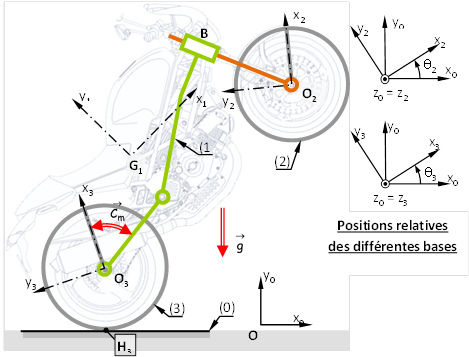
\includegraphics[width=4cm]{images/fig_01}\\
%%\textit{Toupie}
%
%%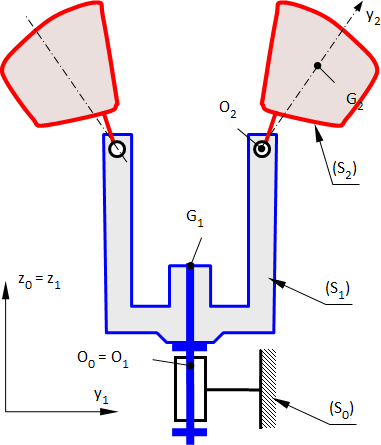
\includegraphics[width=4cm]{images/fig_02}\\
%%\textit{Volants d'inertie d'un vilebrequin}
%
%}%figues de la page de garde
%
%\def\xxpied{%
%Cycles 4 et 5 -- Modéliser les systèmes mécaniques \\% afin de valider leurs performances.\\
%Cours% deChapitre 1 -- \xxactivite%
%}
%
%\setcounter{secnumdepth}{5}
%%---------------------------------------------------------------------------
%
%
%\begin{document}
%\chapterimage{png/Fond_CIN}
%\pagestyle{empty}


%%%%%%%% PAGE DE GARDE COURS
\ifcours
\begin{tikzpicture}[remember picture,overlay]
\node at (current page.north west)
{\begin{tikzpicture}[remember picture,overlay]
\node[anchor=north west,inner sep=0pt] at (0,0) {\includegraphics[width=\paperwidth]{\thechapterimage}};
\draw[anchor=west] (-2cm,-8cm) node [line width=2pt,rounded corners=15pt,draw=ocre,fill=white,fill opacity=0.6,inner sep=40pt]{\strut\makebox[22cm]{}};
\draw[anchor=west] (1cm,-8cm) node {\huge\sffamily\bfseries\color{black} %
\begin{minipage}{1cm}
\rotatebox{90}{\LARGE\sffamily\textsc{\color{ocre}\textbf{\xxnumpartie}}}
\end{minipage} \hfill
\begin{minipage}[c]{14cm}
\begin{titrepartie}
\begin{flushright}
\renewcommand{\baselinestretch}{1.1} 
\Large\sffamily\textsc{\textbf{\xxpartie}}
\renewcommand{\baselinestretch}{1} 
\end{flushright}
\end{titrepartie}
\end{minipage} \hfill
\begin{minipage}[c]{3.5cm}
{\large\sffamily\textsc{\textbf{\color{ocre} \discipline}}}
\end{minipage} 
 };
\end{tikzpicture}};
\end{tikzpicture}


\begin{tikzpicture}[overlay]
\node[shape=rectangle, 
      rounded corners = .25 cm,
	  draw= ocre,
	  line width=2pt, 
	  fill = ocre!10,
	  minimum width  = 2.5cm,
	  minimum height = 3cm,] at (18cm,0) {};
\node at (17.7cm,0) {\rotatebox{90}{\textbf{\Large\color{ocre}{\classe}}}};
%{};
\end{tikzpicture}

\vspace{3.5cm}

\begin{tikzpicture}[remember picture,overlay]
\draw[anchor=west] (-2cm,-6cm) node {\huge\sffamily\bfseries\color{black} %
\begin{minipage}{2cm}
\begin{center}
\LARGE\sffamily\textsc{\color{ocre}\textbf{\xxactivite}}
\end{center}
\end{minipage} \hfill
\begin{minipage}[c]{15cm}
\begin{titrechapitre}
\renewcommand{\baselinestretch}{1.1} 
\Large\sffamily\textsc{\textbf{\xxnumchapitre}}

\Large\sffamily\textsc{\textbf{\xxchapitre}}
\vspace{.5cm}

\renewcommand{\baselinestretch}{1} 
\normalsize\normalfont
\xxcompetences
\end{titrechapitre}
\end{minipage}  };
\end{tikzpicture}
\vfill

\begin{flushright}
\begin{minipage}[c]{.3\linewidth}
\begin{center}
\xxfigures
\end{center}
\end{minipage}\hfill
\begin{minipage}[c]{.6\linewidth}
\startcontents
\printcontents{}{1}{}
\end{minipage}
\end{flushright}

\begin{tikzpicture}[remember picture,overlay]
\draw[anchor=west] (4.5cm,-.7cm) node {
\begin{minipage}[c]{.2\linewidth}
\begin{flushright}

\includegraphics[width=2cm]{png/logoCC}
\end{flushright}
\end{minipage}
\begin{minipage}[c]{.2\linewidth}
\textsl{\xxauteur} \\
\textsl{\classe}
\end{minipage}
 };
\end{tikzpicture}
\newpage
\pagestyle{fancy}

\newpage
\pagestyle{fancy}

\else
\fi


%%%%%%%% PAGE DE GARDE TD
\iftd
%\begin{tikzpicture}[remember picture,overlay]
%\node at (current page.north west)
%{\begin{tikzpicture}[remember picture,overlay]
%\draw[anchor=west] (-2cm,-3.25cm) node [line width=2pt,rounded corners=15pt,draw=ocre,fill=white,fill opacity=0.6,inner sep=40pt]{\strut\makebox[22cm]{}};
%\draw[anchor=west] (1cm,-3.25cm) node {\huge\sffamily\bfseries\color{black} %
%\begin{minipage}{1cm}
%\rotatebox{90}{\LARGE\sffamily\textsc{\color{ocre}\textbf{\xxnumpartie}}}
%\end{minipage} \hfill
%\begin{minipage}[c]{13.5cm}
%\begin{titrepartie}
%\begin{flushright}
%\renewcommand{\baselinestretch}{1.1} 
%\Large\sffamily\textsc{\textbf{\xxpartie}}
%\renewcommand{\baselinestretch}{1} 
%\end{flushright}
%\end{titrepartie}
%\end{minipage} \hfill
%\begin{minipage}[c]{3.5cm}
%{\large\sffamily\textsc{\textbf{\color{ocre} \discipline}}}
%\end{minipage} 
% };
%\end{tikzpicture}};
%\end{tikzpicture}

%%%%%%%%%% PAGE DE GARDE TD %%%%%%%%%%%%%%%
%\begin{tikzpicture}[overlay]
%\node[shape=rectangle, 
%      rounded corners = .25 cm,
%	  draw= ocre,
%	  line width=2pt, 
%	  fill = ocre!10,
%	  minimum width  = 2.5cm,
%	  minimum height = 2.5cm,] at (18.5cm,0) {};
%\node at (17.7cm,0) {\rotatebox{90}{\textbf{\Large\color{ocre}{\classe}}}};
%%{};
%\end{tikzpicture}

% PARTIE ET CHAPITRE
%\begin{tikzpicture}[remember picture,overlay]
%\draw[anchor=west] (-1cm,-2.1cm) node {\large\sffamily\bfseries\color{black} %
%\begin{minipage}[c]{15cm}
%\begin{flushleft}
%\xxnumchapitre \\
%\xxchapitre
%\end{flushleft}
%\end{minipage}  };
%\end{tikzpicture}

% Bandeau titre exo
\begin{tikzpicture}[remember picture,overlay]
\draw[anchor=west] (-2cm,-4cm) node {\huge\sffamily\bfseries\color{black} %
\begin{minipage}{5cm}
\begin{center}
\LARGE\sffamily\color{ocre}\textbf{\textsc{\xxactivite}}

\begin{center}
\xxfigures
\end{center}

\end{center}
\end{minipage} \hfill
\begin{minipage}[c]{12cm}
\begin{titrechapitre}
\renewcommand{\baselinestretch}{1.1} 
\large\sffamily\textbf{\textsc{\xxtitreexo}}

\small\sffamily{\textbf{\textit{\color{black!70}\xxsourceexo}}}
\vspace{.5cm}

\renewcommand{\baselinestretch}{1} 
\normalsize\normalfont
\xxcompetences
\end{titrechapitre}
\end{minipage}  };
\end{tikzpicture}

\else
\fi


%%%%%%%% PAGE DE GARDE FICHE
\iffiche
\begin{tikzpicture}[remember picture,overlay]
\node at (current page.north west)
{\begin{tikzpicture}[remember picture,overlay]
\draw[anchor=west] (-2cm,-3.25cm) node [line width=2pt,rounded corners=15pt,draw=ocre,fill=white,fill opacity=0.6,inner sep=40pt]{\strut\makebox[22cm]{}};
\draw[anchor=west] (1cm,-3.25cm) node {\huge\sffamily\bfseries\color{black} %
\begin{minipage}{1cm}
\rotatebox{90}{\LARGE\sffamily\textsc{\color{ocre}\textbf{\xxnumpartie}}}
\end{minipage} \hfill
\begin{minipage}[c]{14cm}
\begin{titrepartie}
\begin{flushright}
\renewcommand{\baselinestretch}{1.1} 
\large\sffamily\textsc{\textbf{\xxpartie} \\} 

\vspace{.2cm}

\normalsize\sffamily\textsc{\textbf{\xxnumchapitre -- \xxchapitre}}
\renewcommand{\baselinestretch}{1} 
\end{flushright}
\end{titrepartie}
\end{minipage} \hfill
\begin{minipage}[c]{3.5cm}
{\large\sffamily\textsc{\textbf{\color{ocre} \discipline}}}
\end{minipage} 
 };
\end{tikzpicture}};
\end{tikzpicture}


\begin{tikzpicture}[overlay]
\node[shape=rectangle, 
      rounded corners = .25 cm,
	  draw= ocre,
	  line width=2pt, 
	  fill = ocre!10,
	  minimum width  = 2.5cm,
	  minimum height = 2.5cm,] at (18.5cm,0.5cm) {};
%	  minimum height = 2.5cm,] at (18.5cm,0cm) {};
\node at (17.7cm,0.5) {\rotatebox{90}{\textsf{\textbf{\large\color{ocre}{\classe}}}}};
%{};
\end{tikzpicture}



\else
\fi



%\setlength{\columnseprule}{.1pt}
%
%\vspace{2cm}
%\pagestyle{fancy}
%\thispagestyle{plain}
%%%%%%%%%%%%%%%%%%%%%%%%%%%%%%%%%%%%ù




\section{Caractéristiques d'inertie des solides}
L'inertie d'un solide peut se << caractériser >> par la résistance ressentie lorsqu'on souhaite mettre un solide en mouvement. Pour un mouvement de translation, la connaissance de la masse permet de déterminer l'effort nécessaire à la mettre en mouvement. 
Pour un mouvement de rotation, il est nécessaire de connaître la répartition de la masse autour de l'axe de rotation.
%
%\begin{exemple}~\\
%%
%%\begin{itemize}
%%\item Couple pour faire tourner une hélice bipale, tripale, quadripale.
%%\item Couple pour faire tourner une bille et effort pour faire translater une bille.
%%\end{itemize}
%\end{exemple}

\subsection{Détermination de la masse d'un solide}
\subsubsection{Définition}
\begin{defi}[Masse d'un système matériel]~\\
%
On peut définir la masse $M$ d'un système matériel (solide) $S$ par : 
\begin{multicols}{2}
\vspace{-1cm}
$$ M = \int\limits_S \dd m =\int\limits_{P\in V} \mu(P) \dd v $$ 
avec :
\begin{itemize}
\item $\mu(P)$ la masse volumique au point $P$;
\item $\dd v$ un élément volumique de $S$.
\end{itemize}
\end{multicols}
\vspace{.01cm}
\end{defi}
\subsubsection{Principe de conservation de la masse}

\subsection{Centre d'inertie d'un solide}
\subsubsection{Définition}

\begin{defi}[Centre d'inertie d'un solide]
La position du centre d'inertie $G$ d'un solide $S$ est définie par $\int\limits_{P\in S} \vect{GP} \dd m = \vect{0}$.
\end{defi}

Pour déterminer la position du centre d'inertie d'un solide $S$, on passe généralement par l'origine du repère associé à $S$. On a alors 
$\int\limits_{P\in S} \vect{GP} \, \dd m=\int\limits_{P\in S} \left(\vect{GO}+\vect{OP}\right) \dd m = \vect{0} 
\Leftrightarrow \int\limits_{P\in S} \vect{OG} \,\dd m =\int\limits_{P\in S} \vect{OP} \,\dd m
\Leftrightarrow  M\vect{OG} =\int\limits_{P\in S} \vect{OP} \,\dd m$.

\begin{methode}
Pour déterminer les coordonnées $\left(x_G,y_G,z_G\right)$ du centre d'inertie $G$ du solide $S$ dans la base $\repere{O}{x}{y}{z}$, on a donc :
\begin{multicols}{2}
$$
\left\{
\begin{array}{l}
M x_G =\mu \int\limits_{P\in S} x_P \,\dd V \\
M y_G =\mu \int\limits_{P\in S} y_P \,\dd V \\
M z_G =\mu \int\limits_{P\in S} z_P \,\dd V \\
\end{array}
\right. 
$$
avec : 
\begin{itemize}
  \item $\dd V$ : un élément volumique de $S$;
  \item $\mu$ : la masse volumique supposée constante.
\end{itemize}
Pour simplifier les calculs, on peut noter que le centre d'inertie appartient au(x) éventuel(s) plan(s) de symétrie du solide.

\end{multicols}



\end{methode}

\subsubsection{Centre d'inertie d'un solide constitué de plusieurs solides}
Soit un solide composé de $n$ solides élémentaires dont la position des centres d'inertie $G_i$ et les masses $M_i$ sont connues. On note $M=\sum\limits_{i=1}^{n}M_i$.  La position du centre d'inertie $G$ de l'ensemble $S$ est donné par :
$$\vect{OG}=\dfrac{1}{M}\sum\limits_{i=1}^{n}M_i \vect{OG_i} .$$


\subsubsection{Théorème de Guldin}
\paragraph{Centre d'inertie d'une courbe plane}
\paragraph{Centre d'inertie d'une surface plane}

\subsection{Grandeurs inertielles d'un solide}
\subsubsection{Moment et produit d'inertie}
\begin{defi}[Moment d'inertie par rapport à un point dans $\mathcal{R}$]
Soit un repère $\rep{}$ $\repere{O}{i}{j}{k}$ et un point $P$ de coordonnées $\left(x,y,z\right)$ dans $\mathcal{R}$.  
On appelle moment d'inertie du solide $S$ par rapport à un point $O$ la quantité :

$$ I_O(S)=\int\limits_S \vect{OP}^2 \dd m = \int\limits_S \left( x^2 + y^2 + z^2 \right) \dd m.  $$

\end{defi}

\begin{defi}[Moment d'inertie par rapport à un axe dans $\mathcal{R}$]
On appelle moment d'inertie du solide $S$ par rapport à une droite $\left(\Delta\right)$ la quantité positive :

$$ I_{\Delta}(S)=\int\limits_S \left( \vect{\delta} \wedge \vect{AP}\right)^2 \dd m  $$.

Par suite, le moment d'inertie du solide $S$ par rapport à la droite $\left(O,\vect{x}\right)$ est donné par : 
$$ I_{\left(O,\vect{x}\right)}(S)=\int\limits_S \left( \vect{x} \wedge \vect{OP}\right)^2 \dd m.  $$

On détermine donc les moments d'inerties par rapport à $\left(O,\vect{x}\right)$, $\left(O,\vect{y}\right)$ et $\left(O,\vect{z}\right)$ :

$$ I_{\left(O,\vect{x}\right)}(S) =\int\limits_S \left(y^2 + z^2\right) \dd m\quad \quad
I_{\left(O,\vect{y}\right)}(S)     =\int\limits_S \left(x^2 + z^2\right) \dd m\quad \quad
I_{\left(O,\vect{z}\right)}(S)     =\int\limits_S \left(x^2 + y^2\right)\dd m.
$$



\end{defi}

%\begin{defi}[Moment d'inertie par rapport à un point]
%On appelle moment d'inertie du solide $S$ par rapport à un point $A$ la quantité positive :
%
%\begin{tabular}{m{.45\linewidth}m{.45\linewidth}}
%$$ I_A(S)=\int\limits_S \vect{AP}^2 \dd m  $$ &  
%avec :
%\begin{itemize}
%\item $ I_A(S)$ en $\text{kg m}^2$;
%\item $S$ un solide;
%\item $A$ un point;
%\item $P$ un point du solide;
%\item $\dd m$ la quantité de matière.
%\end{itemize} \\
%\end{tabular}
%\end{defi}


%\begin{defi}[Moment d'inertie par rapport à une droite]
%On appelle moment d'inertie du solide $S$ par rapport à une droite $\left(\Delta\right)$ la quantité positive :
%
%\begin{tabular}{m{.45\linewidth}m{.45\linewidth}}
%$$ I_{\Delta}(S)=\int\limits_S \left( \vect{\delta} \vect{AP}\right)^2 \dd m  $$ &  
%avec :
%\begin{itemize}
%\item $ I_\Delta(S)$ en $\text{kg m}^2$;
%\item $\vect{\delta}$
%\item $S$ un solide;
%\item $A$ un point;
%\item $P$ un point du solide;
%\item $\dd m$ la quantité de matière.
%\end{itemize} \\
%\end{tabular}
%\end{defi}

\subsubsection{Matrice d'inertie \label{def_inert}}

\begin{defi}[Matrice d'inertie]
Soient : 
\begin{itemize}
\item un solide $S$ de masse $m$ en mouvement par rapport à un repère $\mathcal{R}_0=\repere{O_0}{i}{j}{k}$;
\item $\mathcal{R}_S=\repere{O}{i}{j}{k}$ le repère lié au solide $S$;
\item $P$ un point de $S$ tel que $\vect{OP}=x_p\vect{i}+y_p\vect{j}+z_p\vect{k}$;
\item $\vect{u}$ un vecteur unitaire du solide $S$.
\end{itemize}

On appelle opérateur d'inertie l'application linéaire définie par :
$$
\vect{u} \rightarrow \vect{J_{\left(O,S\right)}\left(\vect{u}\right)} 
= \int\limits_{S} \vect{OP}\wedge \left(\vect{u}\wedge \vect{OP}\right)\,\dd m
$$

On appelle matrice d'inertie du solide $S$ en $O$, $\inertie{O}{S}$, l'image de cette application linéaire : $\vect{J_{\left(O,S\right)}\left(\vect{u}\right)}  = \inertie{O}{S} \vect{u}$.
 
\end{defi}


Recherchons la matrice de l'application linéaire. On note $\vect{u}=u_x\vect{i}+u_y\vect{j}+u_z\vect{k}$ .
Calculons :$\vect{OP}\wedge \left(\vect{u}\wedge \vect{OP}\right)$.
$$
\begin{bmatrix}
x_p \\ y_p \\ z_p
\end{bmatrix}
\wedge
\left(
\begin{bmatrix}
u_x \\ u_y \\ u_z
\end{bmatrix}
\wedge
\begin{bmatrix}
x_p \\ y_p \\ z_p
\end{bmatrix}
\right)
=
\begin{bmatrix}
x_p \\ y_p \\ z_p
\end{bmatrix}
\wedge
\begin{bmatrix}
u_y z_p - y_p u_z \\
-u_x z_p + x_p u_z \\
u_x y_p - x_p u_y \\
\end{bmatrix}
=
\begin{bmatrix}
 y_p \left( u_x y_p - x_p u_y\right)
 -z_p \left( -u_x z_p + x_p u_z \right) \\
 -x_p \left(u_x y_p - x_p u_y \right)
 +z_p \left(u_y z_p - y_p u_z \right) \\
 x_p \left( -u_x z_p + x_p u_z\right)
 -y_p \left( u_y z_p - y_p u_z\right)
\end{bmatrix}
$$

$$
=
\begin{bmatrix}
  y_p^2 u_x  - y_p x_p u_y   +  z_p^2 u_x  -z_p x_p u_z  \\
   -x_p  y_p u_x+x_p^2 u_y  + z_p^2 u_y  - z_p y_p u_z  \\
   -x_p  z_p u_x+ x_p^2 u_z   -y_p  z_pu_y +y_p^2  u_z
\end{bmatrix}
=
\begin{bmatrix}
 y_p^2 +  z_p^2 &  - y_p x_p &      -x_p  z_p   \\
 -x_p  y_p  & x_p^2   + z_p^2   & - z_p y_p   \\
  -x_p  z_p &    -y_p  z_p  & y_p^2  + x_p^2 
\end{bmatrix}
\begin{bmatrix}
u_x \\ u_y \\ u_z
\end{bmatrix}
$$


\begin{defi}[Matrice d'inertie]
La matrice d'inertie s'écrit ainsi : 
$$
\inertie{O}{S}=\matinertie{\int\limits_{S} \left(y_p^2 + z_p^2 \right)\,\dd m}{\int\limits_{S} \left(x_p^2 + z_p^2 \right)\,\dd m}{\int\limits_{S} \left(x_p^2 + y_p^2 \right)\,\dd m}{-\int\limits_{S} \left(y_pz_p\right)\,\dd m}{-\int\limits_{S} \left(x_pz_p\right)\,\dd m}{-\int\limits_{S} \left(x_py_p\right)\,\dd m}{\mathcal{R}_S}=\matinertie{A}{B}{C}{-D}{-E}{-F}{\mathcal{R}_S}
.$$

On appelle moments d'inertie par rapport aux axes $\axe{O}{{i}}$, $\axe{O}{{j}}$ et $\axe{O}{{k}}$  les termes $A$, $B$ et $C$. 

On appelle produits d'inertie par rapport aux plans $\left(O, \vect{j}, \vect{k}\right)$, $\left(O, \vect{k}, \vect{i}\right)$ et $\left(O, \vect{i}, \vect{j}\right)$ 
les termes $D$, $E$ et $F$.
\end{defi}

\subsubsection{Propriétés des matrices d'inertie}
\subsubsection{Théorème de Huygens}
\begin{theoreme}[Théorème de Huygens]
Le moment d'inertie d'un solide par rapport à un axe  $\axe{A}{\delta}$ est donné par :

\begin{tabular}{m{.45\linewidth}m{.45\linewidth}}
$$I_{\axe{A}{\delta}}(S)=I_{\axe{G}{\delta}}(S)+md^2 $$ & 
avec :
\begin{itemize}
\item $d$ : distance séparant $\axe{A}{\delta}$ et $\axe{G}{\delta}$ en m;
\item $m$ : masse de $S$ en kg.
\end{itemize}
\end{tabular}
\end{theoreme}



\begin{theoreme}[Théorème de Huygens]
Soit $S$ un solide de centre d'inertie $G$, de masse $m$, d'inertie $\inertie{G}{S}$ et d'inertie $\inertie{O}{S}$ avec $\vect{OG}=a\vect{x}+b\vect{y}+c\vect{z}$. Les matrices $\inertie{G}{S}$ et $\inertie{O}{S}$ exprimées dans la base $\mathcal{B}=\base{x}{y}{z}$ sont liées par : 
$$
\matinertie{A_O}{B_O}{C_O}{-D_O}{-E_O}{-F_O}{\mathcal{B}}
= \matinertie{A_G}{B_G}{C_G}{-D_G}{-E_G}{-F_G}{\mathcal{B}}
+ \matinertie{m\left(b^2+c^2\right)}{m\left(a^2+c^2\right)}{m\left(a^2+b^2\right)}{-mbc}{-mac}{-mab}{\mathcal{B}}.
$$


Si le solide est modélisé par une masse ponctuelle $m$ en $G$ et si on souhaite connaître le moment d'inertie pour un point situé à une distance $d$ de $G$, on a $I=md^2$.

\end{theoreme}

\paragraph*{Démonstration}

Par définition, 
$\vect{J_{\left(O,S\right)}\left(\vect{u}\right)} 
= \int\limits_{S} \vect{OP}\wedge \left(\vect{u}\wedge \vect{OP}\right)\,\dd m
$. 

En introduisant le point $G$, on a 
$\vect{J_{\left(O,S\right)}\left(\vect{u}\right)} 
= \int\limits_{S} \left(\vect{OG}+\vect{GP} \right) \wedge \left(\vect{u}\wedge \left(\vect{OG}+\vect{GP} \right) \right)\,\dd m
= \int\limits_{S} \left(\vect{OG}+\vect{GP} \right) \wedge \left(\vect{u}\wedge\vect{OG}+\vect{u}\wedge \vect{GP} \right)\,\dd m
$
 
$= \int\limits_{S} \left(\vect{OG} \wedge \left(\vect{u}\wedge\vect{OG}+\vect{u}\wedge \vect{GP} \right) +\vect{GP}\wedge \left(\vect{u}\wedge\vect{OG}+\vect{u}\wedge \vect{GP} \right) \right) \,\dd m
$ 

$= \int\limits_{S} \left(\vect{OG} \wedge \left(\vect{u}\wedge\vect{OG}\right) +\vect{OG} \wedge \left(\vect{u}\wedge \vect{GP} \right) \right) \,\dd m+ \int\limits_{S} \left( \vect{GP}\wedge \left(\vect{u}\wedge\vect{OG}\right)+\vect{GP}\wedge \left(\vect{u}\wedge \vect{GP} \right) \right) \,\dd m
$ 


$= \int\limits_{S} \left(\vect{OG} \wedge \left(\vect{u}\wedge\vect{OG}\right) \right) \,\dd m
+\int\limits_{S} \left(\vect{OG} \wedge \left(\vect{u}\wedge \vect{GP} \right) \right) \,\dd m
+\int\limits_{S} \left( \vect{GP}\wedge \left(\vect{u}\wedge\vect{OG}\right)\right) \,\dd m
+\int\limits_{S} \left(\vect{GP}\wedge \left(\vect{u}\wedge \vect{GP} \right) \right) \,\dd m
$ 

$= \vect{J_{\left(G,S\right)}\left(\vect{u}\right)} 
+ \vect{OG} \wedge \left(\vect{u}\wedge \int\limits_{S}\vect{GP} \,\dd m\right) 
+\int\limits_{S} \left( \vect{GP}\right) \,\dd m\wedge \left(\vect{u}\wedge\vect{OG}\right)
+ \left(\vect{GP}\wedge \left(\vect{u}\wedge \vect{GP} \right) \right) \int\limits_{S}\,\dd m
$ 

$G$ étant le centre d'inertie du solide, on a $\vect{GP} \,\dd m=\vect{0}$ (par défintion du centre d'inertie). 

En conséquences, $ \vect{J_{\left(O,S\right)}\left(\vect{u}\right)} = \vect{J_{\left(G,S\right)}\left(\vect{u}\right)} 
+ \left(\vect{GP}\wedge \left(\vect{u}\wedge \vect{GP} \right) \right) \int\limits_{S}\,\dd m
$ 

On note $\vect{GP}=a\vect{i}+b\vect{j}+c\vect{k}$ et $M_S=\int\limits_{S}\,\dd m$.

En reprenant le calcul vu en \ref{def_inert}, on a : 
$\left(\vect{GP}\wedge \left(\vect{u}\wedge \vect{GP} \right) \right) = $
$\begin{bmatrix}
 b^2 +  c^2 &  - ab &      -ac   \\
 -ab  & a^2   +c^2   & - bc   \\
  -ac &    -bc  &   a^2 +b^2 
\end{bmatrix}
\begin{bmatrix}
u_x \\ u_y \\ u_z
\end{bmatrix}$. 

\begin{flushright}
\textit{CQFD.}
\end{flushright}


\subsubsection{Rotation de la matrice d'inertie}

\section{Cinétique et dynamique du solide indéformable}
\subsection{Le torseur cinétique}
\subsubsection{Définition}

\begin{defi}[Torseur cinétique]
Le \textbf{torseur cinétique} d'un solide $S$ dans son mouvement par rapport à $R_0$ exprimé en un point $A$ quelconque se définit de la façon suivante,
$$
\torseurcin{C}{S}{R_0}=\torseurl{
\vect{R_c}(S/R_0)=\displaystyle{\int_{P\in S}}\vect{V}(P/R_0)\;\dd m}{\vectmc{A}{S}{R_0}=\displaystyle{\int_{P\in S}}\vect{AP}\wedge \vect{V}(P/R_0)\; \dd m}{A}.
$$
\begin{itemize}
\item La résultante du torseur cinétique $\vect{R_c}(S/R_0)$ s'exprime en $\text{kg m s}^{-1}$ et ne dépend pas du point $A$ mais uniquement du centre d'inertie $G$ de $S$ (de masse $m$) :
$\vectrc{S}{R_0}=m\;\vect{V}(G/R_0)$.

\item Le moment cinétique dépend du point $A$ et peut s'exprimer avec la formule fondamentale de changement de point : $\vectmc{B}{S}{R_0}=\vectmc{A}{S}{R_0}+\vect{BA}\wedge \vect{R_c}(S/R_0)$.
\end{itemize}

\end{defi}

Calculons alors le moment cinétique : 

$\vectmc{A}{S}{R_0}=\int\limits_{P\in S}\vect{AP}\wedge \vectv{P}{S}{R_0}\; \dd m$
$=\int\limits_{P\in S}\vect{AP}\wedge \left( \vectv{A}{S}{R_0} + \vect{PA}\wedge \vecto{S}{R_0} \right)\; \dd m$

$=\int\limits_{P\in S}\vect{AP}\wedge  \vectv{A}{S}{R_0} \; \dd m
+\int\limits_{P\in S}\vect{AP}\wedge \left(  \vect{PA}\wedge \vecto{S}{R_0} \right)\; \dd m$

$=\int\limits_{P\in S}\vect{AP}\wedge  \vectv{A}{S}{R_0} \; \dd m
+\int\limits_{P\in S}\vect{AP}\wedge \left(   \vecto{S}{R_0} \wedge\vect{AP} \right)\; \dd m$


On reconnaît l'opérateur d'inertie : $\int\limits_{P\in S}\vect{AP}\wedge \left(   \vecto{S}{R_0} \wedge\vect{AP} \right)\; \dd m = \inertie{A}{S}\vecto{S}{R_0}$.

On a donc
$\vectmc{A}{S}{R_0}=\int\limits_{P\in S}\vect{AP}\wedge  \vectv{A}{S}{R_0} \; \dd m +\inertie{A}{S}\vecto{S}{R_0}$
$=\int\limits_{P\in S}\vect{AP} \; \dd m  \wedge  \vectv{A}{S}{R_0} +\inertie{A}{S}\vecto{S}{R_0}$.

On reconnaît $\int\limits_{P\in S}\vect{AP} \; \dd m = m \vect{AG}$.

Au final, 
$\vectmc{A}{S}{R_0}=m \vect{AG}  \wedge  \vectv{A}{S}{R_0} +\inertie{A}{S}\vecto{S}{R_0}$.

\subsubsection{Cas particuliers}

\subsection{Le torseur dynamique}
\subsubsection{Définition}
\begin{defi}[Torseur dynamique]
Le \textbf{torseur dynamique} d'un solide $S$ dans son mouvement par rapport à $R_0$ se définit de la façon suivante,

$$
\torseurcin{D}{S}{R_0}=\torseurl{\vect{R_d}(S/R_0)=\displaystyle{\int_{P\in S}}\vect{\Gamma}(P/R_0)\;\dd m}{\vectmd{A}{S}{R_0}=\displaystyle{\int_{P\in S}}\vect{AP}\wedge \vect{\Gamma}(P/R_0)\;\dd m}{A}
$$

\begin{itemize}
\item La résultante du torseur dynamique, $\vect{R_d}(S/R_0)$ ne dépend pas du point $A$ mais uniquement du centre de gravité $G$ de S (de masse $m$) et vérifie :

$$\vect{R_d}(S/R_0)=m\;\vect{\Gamma}(G/R_0).
$$
\item Le moment dynamique dépend du point A et peut s'exprimer avec la formule fondamentale de changement de point :
$$
\vectmd{B}{S}{R_0}=\vectmd{A}{S}{R_0}+\vect{BA}\wedge \vect{R_d}(S/R_0).
$$
\end{itemize}
\end{defi}

Calculons le moment dynamique. Pour cela, commençons par dériver le moment cinétique : 


$\left[ \dfrac{\dd \vectmc{A}{S}{\rep{0}}}{\dd t} \right]_{\rep{0}}=\dfrac{\dd }{\dd t}\left[\int\limits_{P\in S}\vect{AP}\wedge \vectv{P}{S}{\rep{0}}\; \dd m\right]_{\rep{0}}$
$=\int\limits_{P\in S} \dfrac{\dd }{\dd t}\left[ \vect{AP}\wedge \vectv{P}{S}{\rep{0}} \right]_{\rep{0}}\; \dd m$

$=\int\limits_{P\in S} \dfrac{\dd }{\dd t}\left[ \vect{AP} \right]_{\rep{0}}\wedge \vectv{P}{S}{\rep{0}}\; \dd m 
+ \int\limits_{P\in S}  \vect{AP}\wedge \dfrac{\dd }{\dd t}\left[\vectv{P}{S}{\rep{0}} \right]_{\rep{0}}\; \dd m$

$=\int\limits_{P\in S} \dfrac{\dd }{\dd t}\left[ \vect{AO}+\vect{OP} \right]_{\rep{0}}\wedge \vectv{P}{S}{\rep{0}}\; \dd m 
+ \int\limits_{P\in S}  \vect{AP}\wedge \vectg{P}{S}{\rep{0}} \; \dd m$

$=\int\limits_{P\in S} \left(-\vectv{A}{S}{\rep{0}} + \vectv{P}{S}{\rep{0}}\right)\wedge \vectv{P}{S}{\rep{0}}\; \dd m 
+ \int\limits_{P\in S}  \vect{AP}\wedge \vectg{P}{S}{\rep{0}} \; \dd m$

$=\int\limits_{P\in S} \left(\vectv{P}{S}{\rep{0}} \wedge \vectv{P}{S}{\rep{0}}-\vectv{A}{S}{\rep{0}}\wedge \vectv{P}{S}{\rep{0}}  \right)\; \dd m 
+ \int\limits_{P\in S}  \vect{AP}\wedge \vectg{P}{S}{\rep{0}} \; \dd m$

$=-\int\limits_{P\in S} \vectv{A}{S}{\rep{0}}\wedge \vectv{P}{S}{\rep{0}} \; \dd m 
+ \int\limits_{P\in S}  \vect{AP}\wedge \vectg{P}{S}{\rep{0}} \; \dd m$

On a donc 

$ \vectmd{A}{S}{R_0}= \int\limits_{P\in S}  \vect{AP}\wedge \vectg{P}{S}{\rep{0}} \; \dd m = 
\left[ \dfrac{\dd \vectmc{A}{S}{\rep{0}}}{\dd t} \right]_{\rep{0}} + \int\limits_{P\in S} \vectv{A}{S}{\rep{0}}\wedge \vectv{P}{S}{\rep{0}} \; \dd m $.

Par suite, $\int\limits_{P\in S} \vectv{A}{S}{\rep{0}}\wedge \vectv{P}{S}{\rep{0}} \; \dd m =\vectv{A}{S}{\rep{0}}\wedge \int\limits_{P\in S}  \vectv{P}{S}{\rep{0}} \; \dd m  $
$=\vectv{A}{S}{\rep{0}}\wedge m \vectv{G}{S}{\rep{0}} $.

Au final, 

$ \vectmd{A}{S}{R_0}= \left[ \dfrac{\dd \vectmc{A}{S}{\rep{0}}}{\dd t} \right]_{\rep{0}} +m \vectv{A}{S}{\rep{0}}\wedge  \vectv{G}{S}{\rep{0}} $ ou encore 
$ \vectmd{A}{S}{R_0}= \left[ \dfrac{\dd \vectmc{A}{S}{\rep{0}}}{\dd t} \right]_{\rep{0}} + \vectv{A}{S}{\rep{0}}\wedge  \vectrc{S}{\rep{0}} $.

\subsubsection{Cas particuliers}

\subsection{Énergie cinétique}
\subsubsection{Définition}
\subsubsection{Cas du solide indéformable}
\subsubsection{Cas d'un système de solide}
\subsubsection{Inertie équivalente}
\section{Puissance}
\subsection{Puissance d'une action mécanique extérieure à un ensemble matériel}
\begin{defi}%[Puissance d'une action mécanique extérieure à un ensemble matériel]
On définit la \textbf{puissance d'une action mécanique extérieure} à un ensemble matériel $(E)$ en mouvement par rapport à un référentiel $R$ subissant une densité d'effort $\vect{f}(M)$ (où $M$ est un point courant de $(E)$) comme :

$$
\mathcal{P}(\text{ext} \rightarrow E/R)=\displaystyle{\int_{M\in E}}\vect{f}(M)\cdot \vectv{M}{E}{R}%(M\in E/R)%\vect{V}(M\in E/R)
\dd V.
$$
\end{defi}

\begin{rem}%%[Puissance galiléenne]
On appellera \textbf{puissance galiléenne}, la puissance d'un ensemble matériel $(E)$ en mouvement dans un \textbf{référentiel galiléen} $R_g$ : 
%\begin{align}
%\boxed{
$
\mathcal{P}(\text{ext} \rightarrow E/R_g)
$.
%}
%\end{align}
\end{rem}%


\begin{warn}\textbf{Dimensions et homogénéité.}
\begin{itemize}
\item Une puissance est une \textbf{grandeur scalaire} s'exprimant en \textit{Watt}.
\item Elle est homogène à un produit entre un effort et une vitesse et peut donc s'exprimer en unité SI en $\text{Nms}^{-1}$.
\item Historiquement on a utilisé longtemps les << chevaux >> ou << cheval vapeur >> ($\SI{1}{ch}= \SI{736}{W}$).
\end{itemize}

\end{warn}

\begin{prop}[Calcul des actions mécaniques s'appliquant sur un ensemble E]
On considère un ensemble matériel $E$ composé de $n$ solides $S_i$. 

Dans la pratique pour calculer la puissance totale des actions mécaniques s'appliquant sur $E$ dans son mouvement par rapport à $R$ il faut sommer toutes les puissances s'appliquant sur les $S_i$ venant de l'extérieur de $E$ :
$$
\mathcal{P}(\text{ext} \rightarrow E/R)=\displaystyle{\sum_{\forall S_i \in E}\mathcal{P}(\text{ext} \rightarrow S_i/R)}.
$$
\end{prop}

%\begin{exemple}[Application sur le système de dépose de composants]
%On considère l'ensemble $E=\left\{S_1+S_2+S_3\right\}$
%
%\question{Construire le graph des liaisons modélisant le système entier.}
%
%\begin{texteCache}
%\begin{center}
%\includegraphics[width=0.9\textwidth]{../../../../sujets/dynamique/depose_composant/images/graph_structure.png}
%\end{center}
%\end{texteCache}
%
%\question{Déterminer l'expression de $\mathcal{P}(\text{ext} \rightarrow E/R_g)$ en fonction de puissances extérieures élémentaires (on ne développera pas les calculs explicitement pour l'instant).}
%\begin{texteCache}
%\begin{align*}
%\mathcal{P}(\text{ext} \rightarrow E/R_g)=\mathcal{P}(S_0 \rightarrow S_1/R_0)+\mathcal{P}(Moteur \rightarrow S_1/R_0)
%+\mathcal{P}(S_0 \rightarrow S_3/R_0)+\mathcal{P}(poids \rightarrow S_3/R_0)
%\end{align*}
%\end{texteCache}
%\end{exemple}

\subsection{Puissance d'une action mécanique extérieure à un solide}
\begin{defi}[Puissance d'une action mécanique extérieure à un solide $(S)$]
\textbf{La puissance d'une action mécanique extérieure} à un solide $(S)$ en mouvement dans un référentiel $R$ peut s'écrire comme le comoment entre le torseur des actions mécaniques que subit $(S)$ et le torseur cinématique du mouvement de $S$ dans le référentiel $R$.

%\begin{align}\label{puissance_action}
%\boxed{
$$
\mathcal{P}(\text{ext} \rightarrow S/R)=\torseurstat{T}{\text{ext}}{S}\otimes \torseurcin{V}{S}{R}.
$$

En développant l'expression, on a :
$\mathcal{P}(\text{ext} \rightarrow S/R)=\vectf{\text{ext}}{S}\cdot \vectv{P}{S}{R}+ \vectm{P}{\text{ext}}{S}\cdot\vecto{S}{R}$.
%}
%\end{align}
\end{defi}



\begin{warn}
On veillera bien, pour effectuer le \textbf{comoment} de deux torseurs, à les avoir exprimé au préalable {\textbf{en un même point.}}
\end{warn}

\begin{rem}%[Cas particuliers]
\begin{itemize}
\item Le comoment des torseurs est défini par 
$\torseurstat{T}{\text{ext}}{S}\otimes \torseurcin{V}{S}{R}$
$=
\torseurl{\vectf{\text{ext}}{S}}{\vectm{P}{\text{ext}}{S}}{P}
\otimes \torseurl{\vecto{S}{R}}{\vectv{P}{S}{R}}{P}$ 
$=\vectf{\text{ext}}{S}\cdot \vectv{P}{S}{R}+ \vectm{P}{\text{ext}}{S}\cdot\vecto{S}{R}$.

\item Lorsque le torseur cinématique de $S/R$ est un couple (mouvement de translation) alors en tout point $A$ la puissance est alors donnée par
$
\mathcal{P}(\text{ext} \rightarrow S/R)=\vectf{\text{ext}}{S}\cdot \vectv{P}{S}{R} \;
\forall P.
$

\item Lorsque le torseur des actions mécaniques est un torseur couple alors la puissance est donnée par
$
\mathcal{P}(\text{ext} \rightarrow S/R)=\vectm{P}{\text{ext}}{S}\cdot\vecto{S}{R}\;
\forall P.
$

\end{itemize}
\end{rem}%



\subsubsection*{Démonstration}
On a par définition
$ \mathcal{P}(\text{ext} \rightarrow E/R)=\displaystyle{\int_{M\in E}}\vect{f}(M)\cdot \vectv{M}{E}{R} \dd V $.

En exprimant la vitesse au point $M$ en fonction du point $P$ appartenant au solide $E$, on a 
$ \vectv{M}{E}{R} = \vectv{P}{E}{R}  + \vect{MP}\wedge \vecto{E}{R}$.


En conséquence, 

$ \mathcal{P}(\text{ext} \rightarrow E/R)=\displaystyle{\int_{M\in E}}\vect{f}(M)\cdot \left( \vectv{P}{E}{R}  + \vect{MP}\wedge \vecto{E}{R} \right) \dd V $

$ \mathcal{P}(\text{ext} \rightarrow E/R)=\displaystyle{\int_{M\in E}}\vect{f}(M)\cdot  \vectv{P}{E}{R}   \dd V
+\displaystyle{\int_{M\in E}}\vect{f}(M)\cdot \left(  \vect{MP}\wedge \vecto{E}{R} \right) \dd V $.

$P$ étant un point fixe de $E$ et indépendant de $\dd V$, le produit mixte étant invariant par permutation circulaire et $ \vecto{E}{R}$ étant un vecteur indépendant du point d'écriture, on a donc :

$ \mathcal{P}(\text{ext} \rightarrow E/R)
=  \vectv{P}{E}{R} \displaystyle{\int_{M\in E}}\vect{f}(M)  \dd V
+\displaystyle{\int_{M\in E}}\vecto{E}{R}\cdot \left( \vect{f}(M)\wedge  \vect{MP} \right) \dd V $.

$ \mathcal{P}(\text{ext} \rightarrow E/R)
=  \vectv{P}{E}{R} \displaystyle{\int_{M\in E}}\vect{f}(M)  \dd V
+\vecto{E}{R}\cdot \displaystyle{\int_{M\in E}}  \vect{f}(M)\wedge  \vect{MP}  \dd V $.

$ \mathcal{P}(\text{ext} \rightarrow E/R)
=  \vectv{P}{E}{R} \displaystyle{\int_{M\in E}}\vect{f}(M)  \dd V
+\vecto{E}{R}\cdot \displaystyle{\int_{M\in E}}  \vect{PM}\wedge \vect{f}(M)   \dd V $.


Or, $\displaystyle{\int_{M\in E}}\vect{f}(M)  \dd V = \vectf{\text{ext}}{E}$ et 
$ \displaystyle{\int_{M\in E}}  \vect{PM}\wedge \vect{f}(M)   \dd V = \vectm{P}{\text{ext}}{E}$.

En conséquences, 

$ \mathcal{P}(\text{ext} \rightarrow E/R)
=  \vectv{P}{E}{R}\cdot \vectf{\text{ext}}{E} +\vecto{E}{R}\cdot  \vectm{P}{\text{ext}}{E} $.


\subsection{Puissance d'actions mutuelles entre deux solides}


\begin{defi}[Puissance d'actions mutuelles entre deux solides]
Soient deux solides $(S_1)$ et $(S_2)$ distincts, en mouvement par rapport à un référentiel galiléen $R_g$, et exerçant une action mécanique l'un sur l'autre.
\textbf{La puissance} \textbf{des actions mutuelles} entre $(S_1)$ et $(S_2)$, dans leur mouvement par rapport au repère $R$, est :
$$
\mathcal{P}(S_1 \leftrightarrow S_2/R_g)=\mathcal{P}(S_1 \rightarrow S_2/R_g)+\mathcal{P}(S_2 \rightarrow S_1/R_g).
$$		
 
 \end{defi}

\begin{prop}
La \textbf{puissance des actions mutuelles} entre $(S_1)$ et $(S_2)$ \textbf{est indépendante du repère $R$}.
Ainsi,
$$\mathcal{P}(S_1 \leftrightarrow S_2/R)=\mathcal{P}(S_1 \leftrightarrow S_2).
$$
\end{prop}


\begin{rem}%
\begin{itemize}
\item On peut parler parfois de \textbf{puissance des inter-efforts}.
\item Pour un ensemble $E$, on peut exprimer l'ensemble de la puissance des inter-effort comme la puissance intérieure à l'ensemble $E$ : 
$$
\mathcal{P}_{\text{int}}(E)=\displaystyle{\sum^n_{j=1}}\displaystyle{\sum^{j-1}_{i=1}}\mathcal{P}(S_i \leftrightarrow S_j).
$$
\end{itemize}

\end{rem}%


\subsection{Puissances d'actions mutuelles dans les liaisons}
\begin{defi}[Puissances d'actions mutuelles dans les liaisons]
Si deux solides $S_1$ et $S_2$ sont en liaison, on a :
$$
\mathcal{P}(S_1 \leftrightarrow S_2) = \torseurstat{T}{S_1}{S_2}\otimes \torseurcin{V}{S_2}{S_1}.
$$

La \textbf{liaison parfaite} si et seulement si quel que soit le mouvement de $S_2$ par rapport à $S_1$ autorisé par la liaison entre ces deux solides, la \textbf{puissance des actions mutuelles entre $S_1$ et $S_2$ est nulle}.
$$
\mathcal{P}(S_1 \leftrightarrow S_2)=0.
$$
\end{defi}


\begin{rem}%
\begin{itemize}
\item La notion de \textbf{liaison parfaite} s'étend facilement à une liaison équivalente à plusieurs liaisons placées en parallèle et en série entre deux solide $S_1$ et $S_2$. Pour cela il suffit de considérer les torseurs d'action mécanique transmissible et cinématique de la liaison équivalente.
\item L'hypothèse d'une liaison parfaite a pour avantage de mettre en place le théorème de l'énergie cinétique (qui est une conséquence du principe fondamental de la dynamique) sans préjuger de la technologie de la liaison.
\end{itemize}
\end{rem}%


\section{Principe fondamental de la dynamique}

\section{Théorème de l'énergie puissance}

\section{Méthodologie}




%
%\begin{thebibliography}{2}
%   \bibitem[1]{ref1} Émilien Durif, {\it Approche énergétique des systèmes, Lycée La Martinière Monplaisir, Lyon.}
%\end{thebibliography}
%




